\section{Supplementary Material for Evaluation}
\label{sec:supp:evaluation}

\subsection{\fh{Evaluation Prompt Templates}}
\label{sec:supp:evaluation-prompts}

\fh{We provide the evaluation prompt templates for transparency. The standard prompt asks models to produce a structured scientific rationale before the final classification, so the main setting already includes an explicit deliberation-style instruction. The aggressive prompt keeps the same task but changes the default decision rule to require stronger evidence before assigning high soundness.}

\begin{tcolorbox}[title=\textbf{System Prompt for Standard Evaluation}]
\small

You are an expert ML researcher and peer reviewer. Classify the scientific rigor bucket of a research idea and your assessment confidence from 1 to 5 from its hypothesis and experiment description.

Output the assessment as a JSON object, including a detailed step-by-step justification for the rigor bucket selected.

\end{tcolorbox}

\begin{tcolorbox}[title=\textbf{User Prompt for Standard Evaluation}]
\small

Classify this hypothesis-experiment pair into one rigor bucket:
\begin{itemize}[leftmargin=*,itemsep=0pt,topsep=0pt]
    \item \texttt{low}: Weak scientific contribution. Hypothesis is vague or trivial, experiments lack controls or baselines, metrics are weak, or methodology has fundamental flaws.
    \item \texttt{high}: Strong scientific contribution. Hypothesis is clear and meaningful. Experiments are rigorous, controlled, include appropriate baselines/ablations, and use suitable metrics.
\end{itemize}

Confidence Score Scale:
\begin{itemize}[leftmargin=*,itemsep=0pt,topsep=0pt]
    \item 1: You are unable to assess this paper and have alerted the ACs to seek an opinion from different reviewers.
    \item 2: You are willing to defend your assessment, but it is quite likely that you did not understand the central parts of the submission or that you are unfamiliar with some pieces of related work. Math/other details were not carefully checked.
    \item 3: You are fairly confident in your assessment. It is possible that you did not understand some parts of the submission or that you are unfamiliar with some pieces of related work. Math/other details were not carefully checked.
    \item 4: You are confident in your assessment, but not absolutely certain. It is unlikely, but not impossible, that you did not understand some parts of the submission or that you are unfamiliar with some pieces of related work.
    \item 5: You are absolutely certain about your assessment. You are very familiar with the related work and checked the math/other details carefully.
\end{itemize}

\textbf{HYPOTHESIS:} \texttt{\{hypothesis\}}

\textbf{EXPERIMENT:} \texttt{\{experiment\}}

Output format:
\begin{verbatim}
{
  "justification": "<Think step-by-step, provide detailed justification>",
  "rigor_bucket": <"low" or "high">,
  "confidence": <1-5 integer>
}
\end{verbatim}

Constraints:
\begin{itemize}[leftmargin=*,itemsep=0pt,topsep=0pt]
    \item \texttt{rigor\_bucket} must be a choice in [\texttt{"low"}, \texttt{"high"}]
    \item \texttt{confidence} must be an integer in [1, 5]
\end{itemize}
\end{tcolorbox}

\begin{tcolorbox}[title=\textbf{System Prompt for Aggressive Evaluation}]
\small

You are a strict ML area chair applying an aggressive rigor filter. Classify scientific rigor from a hypothesis and experiment description.

Default to ``low'' unless the evidence clearly demonstrates strong scientific rigor with concrete controls, strong baselines, appropriate metrics, and a credible evaluation plan.

Output valid JSON only with a detailed step-by-step justification.

\end{tcolorbox}

\begin{tcolorbox}[title=\textbf{User Prompt for Aggressive Evaluation}]
\small

Classify this hypothesis-experiment pair into one rigor bucket under an aggressive standard:
\begin{itemize}[leftmargin=*,itemsep=0pt,topsep=0pt]
    \item \texttt{low}: choose this unless there is clear, concrete, and compelling evidence of rigorous methodology.
    \item \texttt{high}: only if the plan is explicitly strong on hypothesis clarity, experimental controls, baselines/ablations, metric validity, and methodological credibility.
\end{itemize}

Aggressive policy:
\begin{itemize}[leftmargin=*,itemsep=0pt,topsep=0pt]
    \item Penalize missing controls, vague methods, missing or weak baselines, underspecified metrics, unclear evaluation protocol, or hand-wavy claims.
    \item If information is incomplete or ambiguous, prefer \texttt{low}.
    \item Use \texttt{high} only when justification is unambiguous.
\end{itemize}

Confidence Score Scale:
\begin{itemize}[leftmargin=*,itemsep=0pt,topsep=0pt]
    \item 1: You are unable to assess this paper and have alerted the ACs to seek an opinion from different reviewers.
    \item 2: You are willing to defend your assessment, but it is quite likely that you did not understand the central parts of the submission or that you are unfamiliar with some pieces of related work. Math or other details were not carefully checked.
    \item 3: You are fairly confident in your assessment. It is possible that you did not understand some parts of the submission or that you are unfamiliar with some pieces of related work. Math or other details were not carefully checked.
    \item 4: You are confident in your assessment, but not absolutely certain. It is unlikely, but not impossible, that you did not understand some parts of the submission or that you are unfamiliar with some pieces of related work.
    \item 5: You are absolutely certain about your assessment. You are very familiar with the related work and checked the math or other details carefully.
\end{itemize}

\textbf{HYPOTHESIS:} \texttt{\{hypothesis\}}

\textbf{EXPERIMENT:} \texttt{\{experiment\}}

Output format:
\begin{verbatim}
{
  "justification": "<Think step-by-step, provide detailed justification>",
  "rigor_bucket": <"low" or "high">,
  "confidence": <1-5 integer>
}
\end{verbatim}

Constraints:
\begin{itemize}[leftmargin=*,itemsep=0pt,topsep=0pt]
    \item \texttt{rigor\_bucket} must be a choice in [\texttt{"low"}, \texttt{"high"}]
    \item \texttt{confidence} must be an integer in [1, 5]
\end{itemize}
\end{tcolorbox}

\subsection{Does Scale Resolve the Optimism Bias?}\label{sec:supp:scale-bias}

To isolate the effect of model scale from other factors, such as model family and training recipe, we evaluate six models from the same Qwen3.5 family, ranging from 2B to 122B parameters, under both prompting conditions. Results are shown in Fig.~\ref{fig:scale}.



Under standard prompting, scaling improves high-soundness recall monotonically (71.8\% at 2B to 92.8\% at 35B), but low-soundness recall simultaneously decreases (31.0\% at 2B to 19.2\% at 35B). Larger models become \textit{more} permissive toward weak proposals, not less. This suggests that scale improves general language understanding and pattern recognition, but does not correct the optimism tendency in scientific judgment.

Under aggressive prompting, scale provides no consistent benefit. All six models tend toward near-always-low behavior, with high-soundness recall ranging from 1.4\% (4B) to 32.4\% (27B), showing no monotonic trend with size. Notably, the 27B model achieves better balance than both smaller and larger variants, suggesting that the aggressive prompt interacts non-monotonically with model capacity.



Together, these results indicate that the optimism bias observed in Sec.~\ref{sec:eval:main-results} is not a small-model artifact in this family. It persists with scale under standard prompting and remains unresolved under aggressive prompting at all tested sizes. Reliable scientific soundness judgment likely requires interventions beyond simply using larger models.

\subsection{Is the Optimism Bias Caused by Instruction Tuning?}\label{sec:supp:instruction-tuning-bias}

\begin{figure}[t]
    \centering
    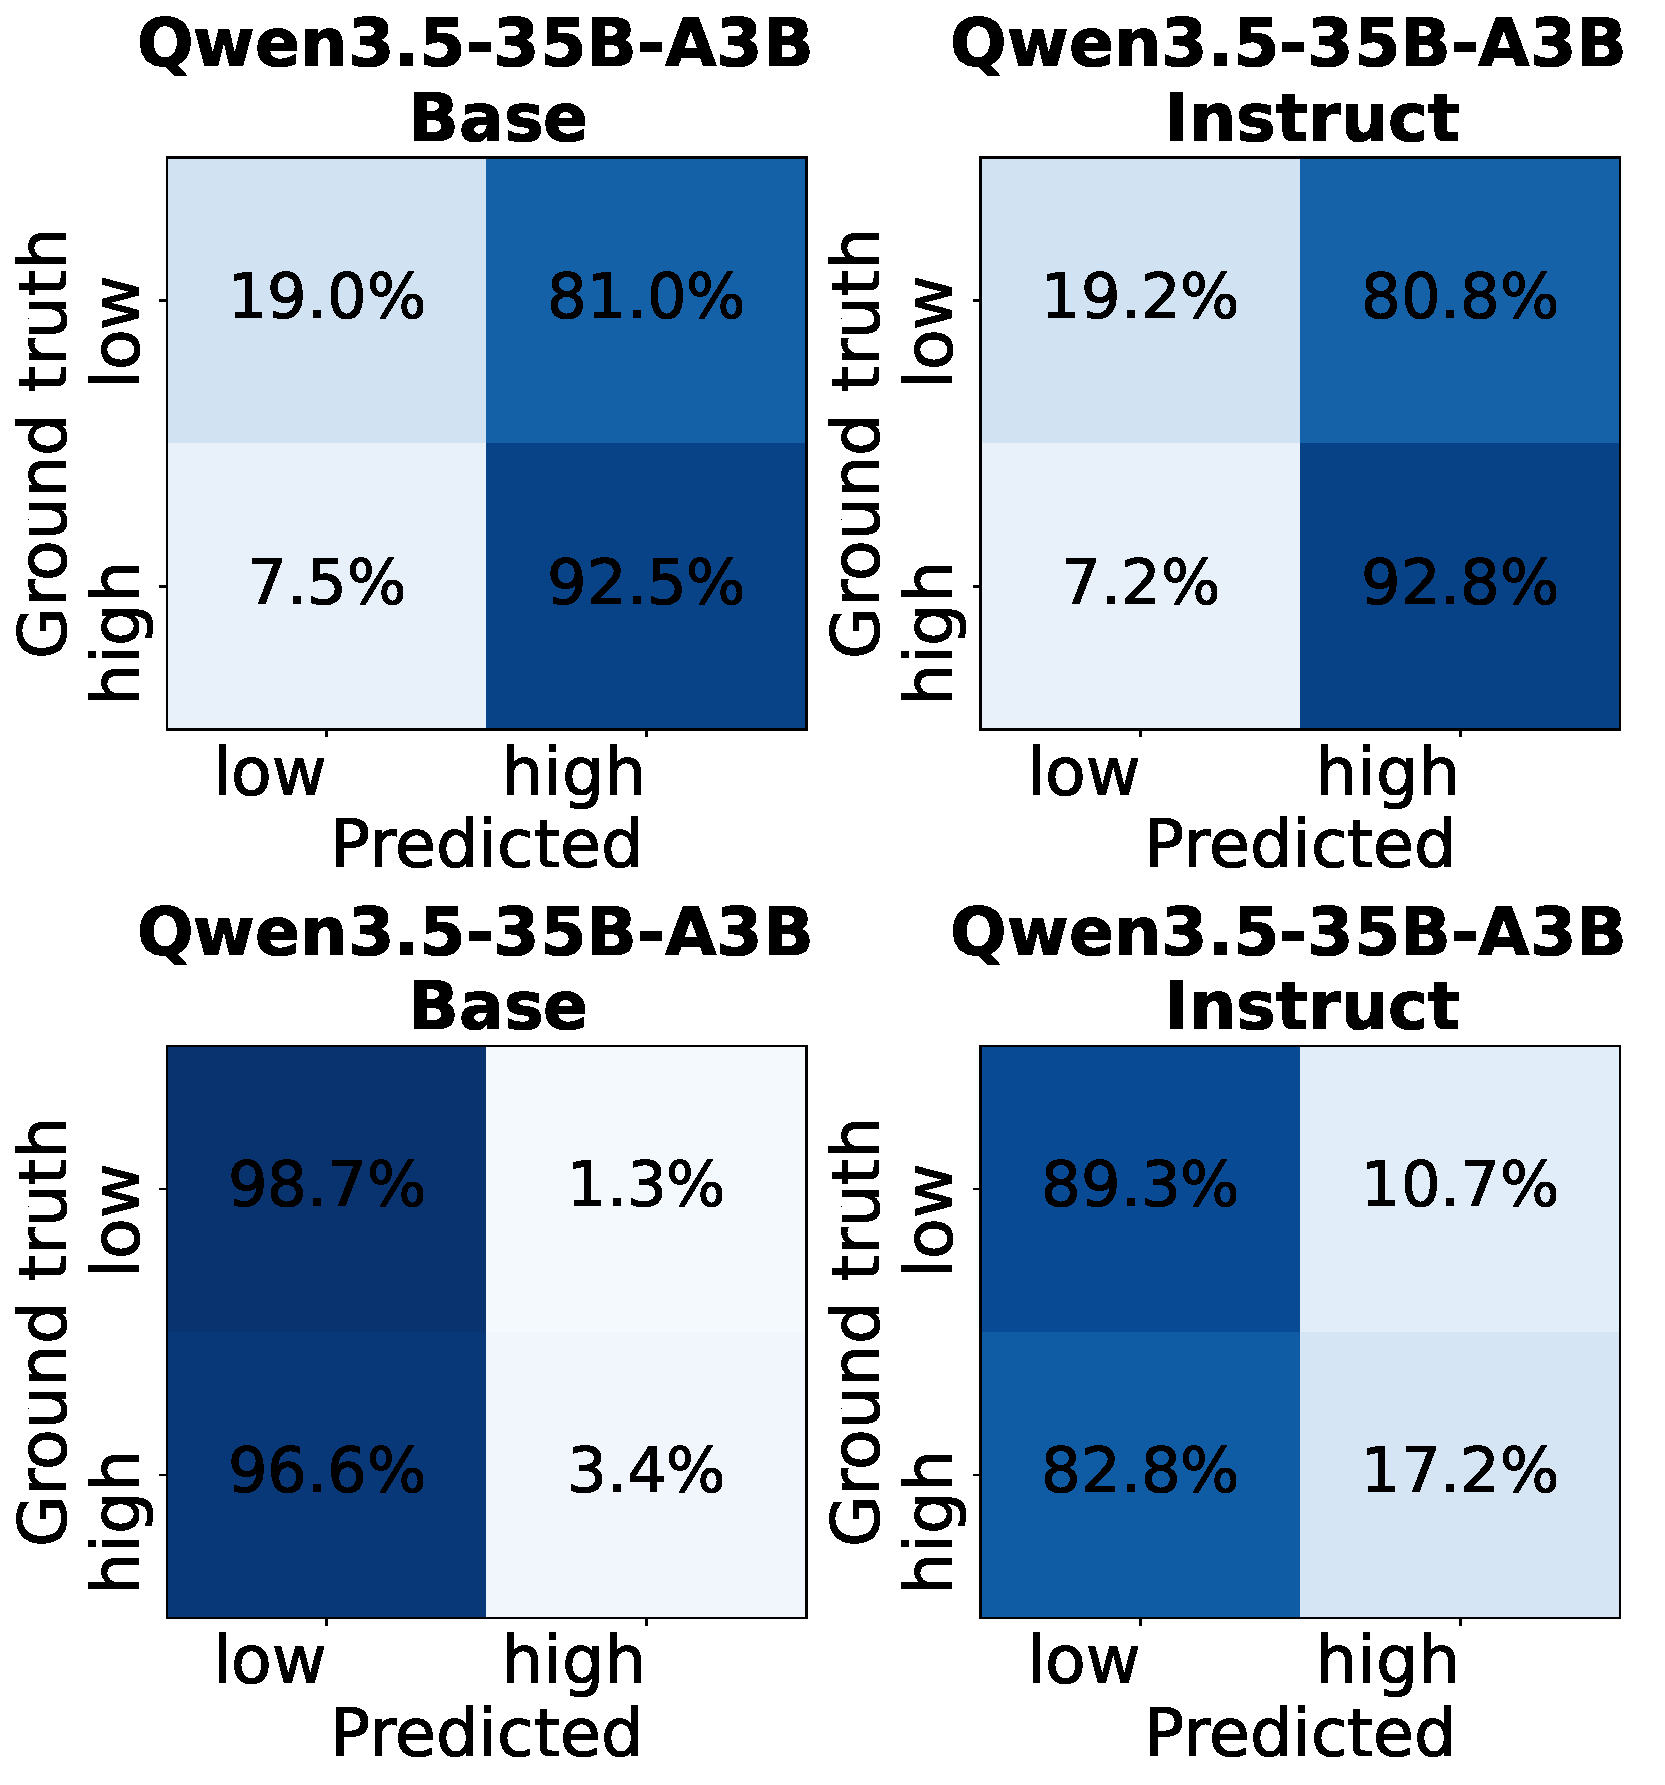
\includegraphics[width=0.55\linewidth]{figures/instruct_confusion_merged.pdf}
    \caption{Base vs.\ instruction-tuned Qwen3.5-35B-A3B under standard \textbf{(top)} and aggressive \textbf{(bottom)} prompting. Under standard prompting, both variants show similar optimism bias, consistent with an origin earlier in training. Under aggressive prompting, the instruction-tuned model is slightly better, but both remain over-conservative.}
    \label{fig:instruct}
\end{figure}

A natural hypothesis is that the optimism bias stems from instruction tuning or RLHF, which may encourage models to be agreeable and avoid negative feedback. To test this, we compare Qwen3.5-35B-A3B in its base and instruction-tuned variants under both prompting conditions, as shown in Fig.~\ref{fig:instruct}.

Under standard prompting, the base and instruction-tuned models are nearly indistinguishable. The base model reaches 19.0\% low-soundness recall and 92.5\% high-soundness recall, while the instruction-tuned model reaches 19.2\% and 92.8\%, respectively. These similar numbers suggest instruction tuning is unlikely to be the sole driver of the optimism bias.

Under aggressive prompting, both models shift toward over-conservatism, but the base model shifts more strongly (98.7\% low recall, 3.4\% high recall) than the instruction-tuned variant (89.3\% low recall, 17.2\% high recall). This suggests instruction tuning may provide modest robustness to prompt pressure, but is insufficient to maintain calibrated judgment.


These findings suggest that resolving the optimism bias may require interventions at or before pre-training (such as targeted training on scientific judgment), rather than relying on post-hoc instruction tuning alone.

\subsection{\fh{Controls for Public-Corpus Contamination}}
\label{sec:supp:contamination-control}

\fh{A natural concern is that ICLR submissions and OpenReview discussions are public, so some evaluated models may have encountered older source papers during pretraining or supervised fine-tuning. We therefore treat contamination as a threat to validity rather than claiming it is fully eliminated. We address it in three ways. First, if a model had memorized acceptance outcomes or reviewer verdicts, that information would likely help it identify low-soundness proposals; the observed high false-positive rate is therefore conservative with respect to our main failure claim. Second, we evaluate an ICLR 2026-only split using a cutoff-restricted model subset with documented training cutoffs before September 2025 where such documentation is available, reducing the chance that these submissions appeared in training data. Third, the identifier-removal analysis in Sec.~\ref{sec:supp:identifier-removal} tests whether recognizable method names or self-identifying phrases drive predictions. As shown in main-text Tab.~\ref{tab:contamination_2026}, the optimism bias is largely stable across the full dataset and the 2026-only split. We will report the exact model-card or technical-report source for each cutoff in the released metadata and exclude models without sufficient cutoff documentation from cutoff-restricted claims.}

\fh{We emphasize that perfect contamination control is difficult for any benchmark built from public corpora. For this reason, we describe this as a reduced-contamination-risk analysis rather than a contamination-free benchmark. SoundnessBench should be interpreted together with the 2026 split, the identifier-removal analysis below, and future private or continuously updated benchmark variants.}

\subsection{\fh{Identifier-Removal Robustness}}
\label{sec:supp:identifier-removal}

\fh{Paper titles are never passed to models in our main evaluation. To further test whether recognizable method names or self-identifying phrases drive the results, we construct an anonymized variant by masking method names, framework names, and self-naming phrases while preserving the scientific meaning of the hypothesis and experiment design. Tab.~\ref{tab:identifier_removal} shows that this intervention has negligible effect on the aggregate confusion matrix, with changes of roughly one percentage point. This suggests that the main behavior is not primarily driven by recognizing paper identities.}

\begin{table}[ht]
\centering
\caption{\fh{Effect of masking paper-identifying phrases. Entries are mean prediction percentages.}}
\label{tab:identifier_removal}
\resizebox{0.65\linewidth}{!}{%
\begin{tabular}{lcc}
\toprule
\fh{\textbf{Ground Truth / Setting}} & \fh{\textbf{Predicted Low}} & \fh{\textbf{Predicted High}} \\
\midrule
\fh{Low (Without Removal)} & \fh{26.12\%} & \fh{73.87\%} \\
\fh{Low (With Removal)} & \fh{25.01\%} & \fh{74.99\%} \\
\fh{High (Without Removal)} & \fh{8.14\%} & \fh{91.86\%} \\
\fh{High (With Removal)} & \fh{8.58\%} & \fh{91.42\%} \\
\bottomrule
\end{tabular}%
}
\end{table}

\subsection{\fh{Surface-Feature Baselines}}
\label{sec:supp:surface-baselines}

\fh{We add simple baselines to test whether shallow structural statistics alone explain the observed behavior. Always-high predicts every proposal as high soundness; always-low predicts every proposal as low soundness. We also evaluate mean-threshold classifiers based on proposal length, experiment count, and risk-factor count, with thresholds set at the midpoint between per-class means. These no-training baselines avoid fitting on the evaluation labels while still probing whether label priors or obvious structural features explain the result. A fully supervised text classifier would answer a different question---how much signal can be learned from labeled SoundnessBench examples---so we leave it to a training-split extension rather than using benchmark test labels for model selection.}

\begin{table}[ht]
\centering
\caption{\fh{Surface-feature and trivial baselines compared with the average LLM under standard prompting.}}
\label{tab:surface_baselines}
\resizebox{\linewidth}{!}{%
\begin{tabular}{lcccc}
\toprule
& \fh{\textbf{Low$\rightarrow$Low}} & \fh{\textbf{Low$\rightarrow$High (FP)}} & \fh{\textbf{High$\rightarrow$Low}} & \fh{\textbf{High$\rightarrow$High}} \\
\midrule
\fh{Always-High} & \fh{0.0\%} & \fh{100.0\%} & \fh{0.0\%} & \fh{100.0\%} \\
\fh{Always-Low} & \fh{100.0\%} & \fh{0.0\%} & \fh{100.0\%} & \fh{0.0\%} \\
\fh{Length Threshold} & \fh{58.5\%} & \fh{41.5\%} & \fh{36.7\%} & \fh{63.3\%} \\
\fh{Experiment Count Threshold} & \fh{64.4\%} & \fh{35.6\%} & \fh{47.7\%} & \fh{52.3\%} \\
\fh{Risk Factor Count Threshold} & \fh{57.4\%} & \fh{42.6\%} & \fh{48.2\%} & \fh{51.8\%} \\
\fh{Avg. LLM (Standard Prompt)} & \fh{\textbf{26.12\%}} & \fh{\textbf{73.87\%}} & \fh{\textbf{8.14\%}} & \fh{\textbf{91.86\%}} \\
\bottomrule
\end{tabular}%
}
\end{table}

\fh{The structural baselines and LLMs fail in qualitatively opposite directions: structural thresholds over-reject high-soundness proposals, whereas LLMs over-approve low-soundness proposals. This divergence suggests that shallow structural statistics alone are insufficient to explain the observed optimism bias, although richer supervised confounder models remain useful future controls.}

\subsection{\fh{Adversarial Injection of Methodological Flaws}}
\label{sec:supp:adversarial-injection}

\fh{To test whether models attend to methodological content at all, we inject targeted flaws into 100 high-soundness proposals. Specifically, dataset names and evaluation metrics are replaced with those from a different domain while keeping the hypothesis and other content fixed, creating severe hypothesis--experiment mismatches. GPT-5.4's approval rate drops from 77.0\% on the original proposals to 1.0\% after injection (Tab.~\ref{tab:adversarial_injection}). This result rules out the strongest version of the inattention hypothesis: the model can detect severe methodological inconsistencies. However, it also sharpens the remaining failure mode: models are still insufficiently critical of subtler naturally occurring flaws in low-soundness proposals. We report this as an initial control and will extend it to more flaw types, such as missing baselines and data leakage, in future benchmark versions.}

\begin{table}[ht]
\centering
\caption{\fh{Adversarial injection of severe methodological mismatches into high-soundness proposals.}}
\label{tab:adversarial_injection}
\resizebox{0.72\linewidth}{!}{%
\begin{tabular}{lccc}
\toprule
\fh{\textbf{Model}} & \fh{\textbf{Original Approval}} & \fh{\textbf{Post-Injection Approval}} & \fh{\textbf{Flip Rate}} \\
\midrule
\fh{GPT-5.4} & \fh{77.0\%} & \fh{1.0\%} & \fh{76.0\%} \\
\bottomrule
\end{tabular}%
}
\end{table}

\subsection{\fh{Breakdowns by Year, Subfield, and Writing Quality}}
\label{sec:supp:slice-breakdowns}

\fh{We further examine whether failures are concentrated in particular years, subfields, or writing-quality bands. Tab.~\ref{tab:year_breakdown}, Tab.~\ref{tab:subfield_breakdown}, and Tab.~\ref{tab:writing_breakdown} report low-soundness false-positive rates. The optimism bias is visible across all slices, suggesting that it is systemic rather than driven by a narrow subset of the benchmark.}

\begin{table}[ht]
\centering
\caption{\fh{Low-soundness false-positive rate by year.}}
\label{tab:year_breakdown}
\resizebox{0.38\linewidth}{!}{%
\begin{tabular}{lc}
\toprule
\fh{\textbf{Year}} & \fh{\textbf{Low-Soundness FP Rate}} \\
\midrule
\fh{2022} & \fh{67.2\%} \\
\fh{2023} & \fh{79.6\%} \\
\fh{2024} & \fh{70.2\%} \\
\fh{2025} & \fh{68.4\%} \\
\fh{2026} & \fh{78.3\%} \\
\fh{All} & \fh{73.87\%} \\
\bottomrule
\end{tabular}%
}
\end{table}

\begin{table}[ht]
\centering
\caption{\fh{Low-soundness false-positive rate by subfield, restricted to subfields with more than 10 pairs.}}
\label{tab:subfield_breakdown}
\resizebox{0.6\linewidth}{!}{%
\begin{tabular}{lc}
\toprule
\fh{\textbf{Subfield}} & \fh{\textbf{Low-Soundness FP Rate}} \\
\midrule
\fh{Reinforcement Learning} & \fh{76.0\%} \\
\fh{Natural Language Processing} & \fh{73.0\%} \\
\fh{Generative Models} & \fh{63.5\%} \\
\fh{Optimization} & \fh{75.3\%} \\
\fh{Representation Learning} & \fh{75.8\%} \\
\fh{Computer Vision} & \fh{76.0\%} \\
\fh{Learning Theory} & \fh{75.6\%} \\
\fh{Graph Neural Networks} & \fh{85.4\%} \\
\fh{All Subfields} & \fh{73.87\%} \\
\bottomrule
\end{tabular}%
}
\end{table}

\begin{table}[ht]
\centering
\caption{\fh{Low-soundness false-positive rate by writing-quality band, using 2024--2026 subset data where presentation scores are available.}}
\label{tab:writing_breakdown}
\resizebox{0.55\linewidth}{!}{%
\begin{tabular}{lc}
\toprule
\fh{\textbf{Writing Quality Band}} & \fh{\textbf{Low-Soundness FP Rate}} \\
\midrule
\fh{Low ($\leq 2$)} & \fh{71.4\%} \\
\fh{Mid ($>2$ and $\leq 3$)} & \fh{81.0\%} \\
\fh{High ($>3$)} & \fh{76.7\%} \\
\fh{All} & \fh{73.87\%} \\
\bottomrule
\end{tabular}%
}
\end{table}





\pagebreak

\subsection{\tuyen{Qualitative Examples of False and True Positives}}
\label{sec:supp:qualitative-fp-tp}

We include representative qualitative examples to illustrate what the aggregate confusion matrices count as false positives and true positives. In Figs.~\ref{fig:example-fp} and~\ref{fig:example-fp-2}, the proposals have low mean ICLR soundness scores but are still predicted as high soundness by the evaluated models, illustrating the optimism-bias failure mode. In Fig.~\ref{fig:example-tp}, the proposal has a high mean ICLR soundness score and is correctly predicted as high soundness, illustrating a true-positive case. We show the corresponding Gemini 3.1 Pro, GPT-5.4 Thinking, and Claude Opus 4.6 responses below each proposal.

\begin{figure}[p]
    \centering
    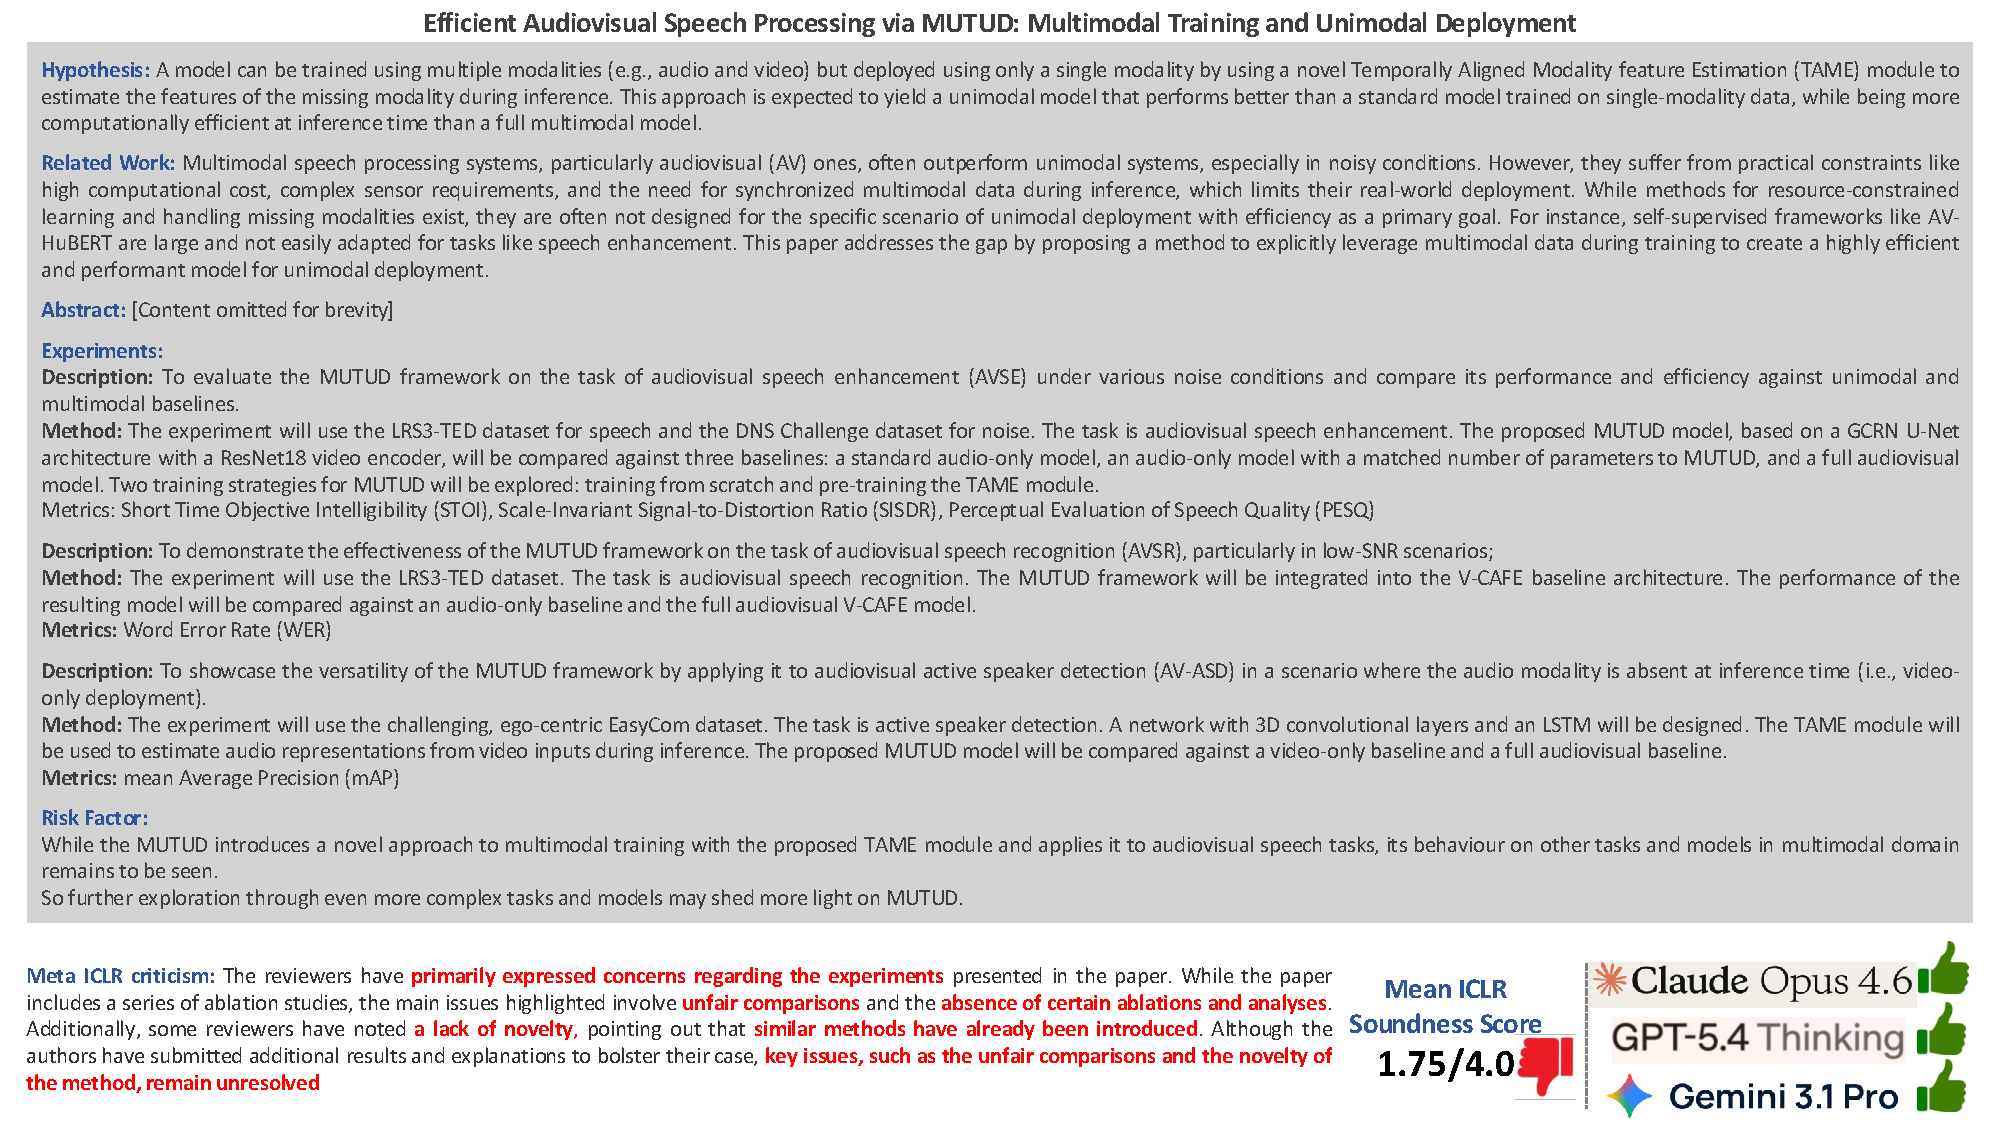
\includegraphics[width=\linewidth]{figures/example-fp.pdf}
    \caption{\textbf{False-positive example.} A low-soundness proposal is predicted as high soundness by Claude Opus 4.6, GPT-5.4 Thinking, and Gemini 3.1 Pro despite reviewer concerns about the experimental comparisons, missing ablations or analyses, and novelty.}
    \label{fig:example-fp}
\end{figure}

\begin{figure}[p]
    \centering
    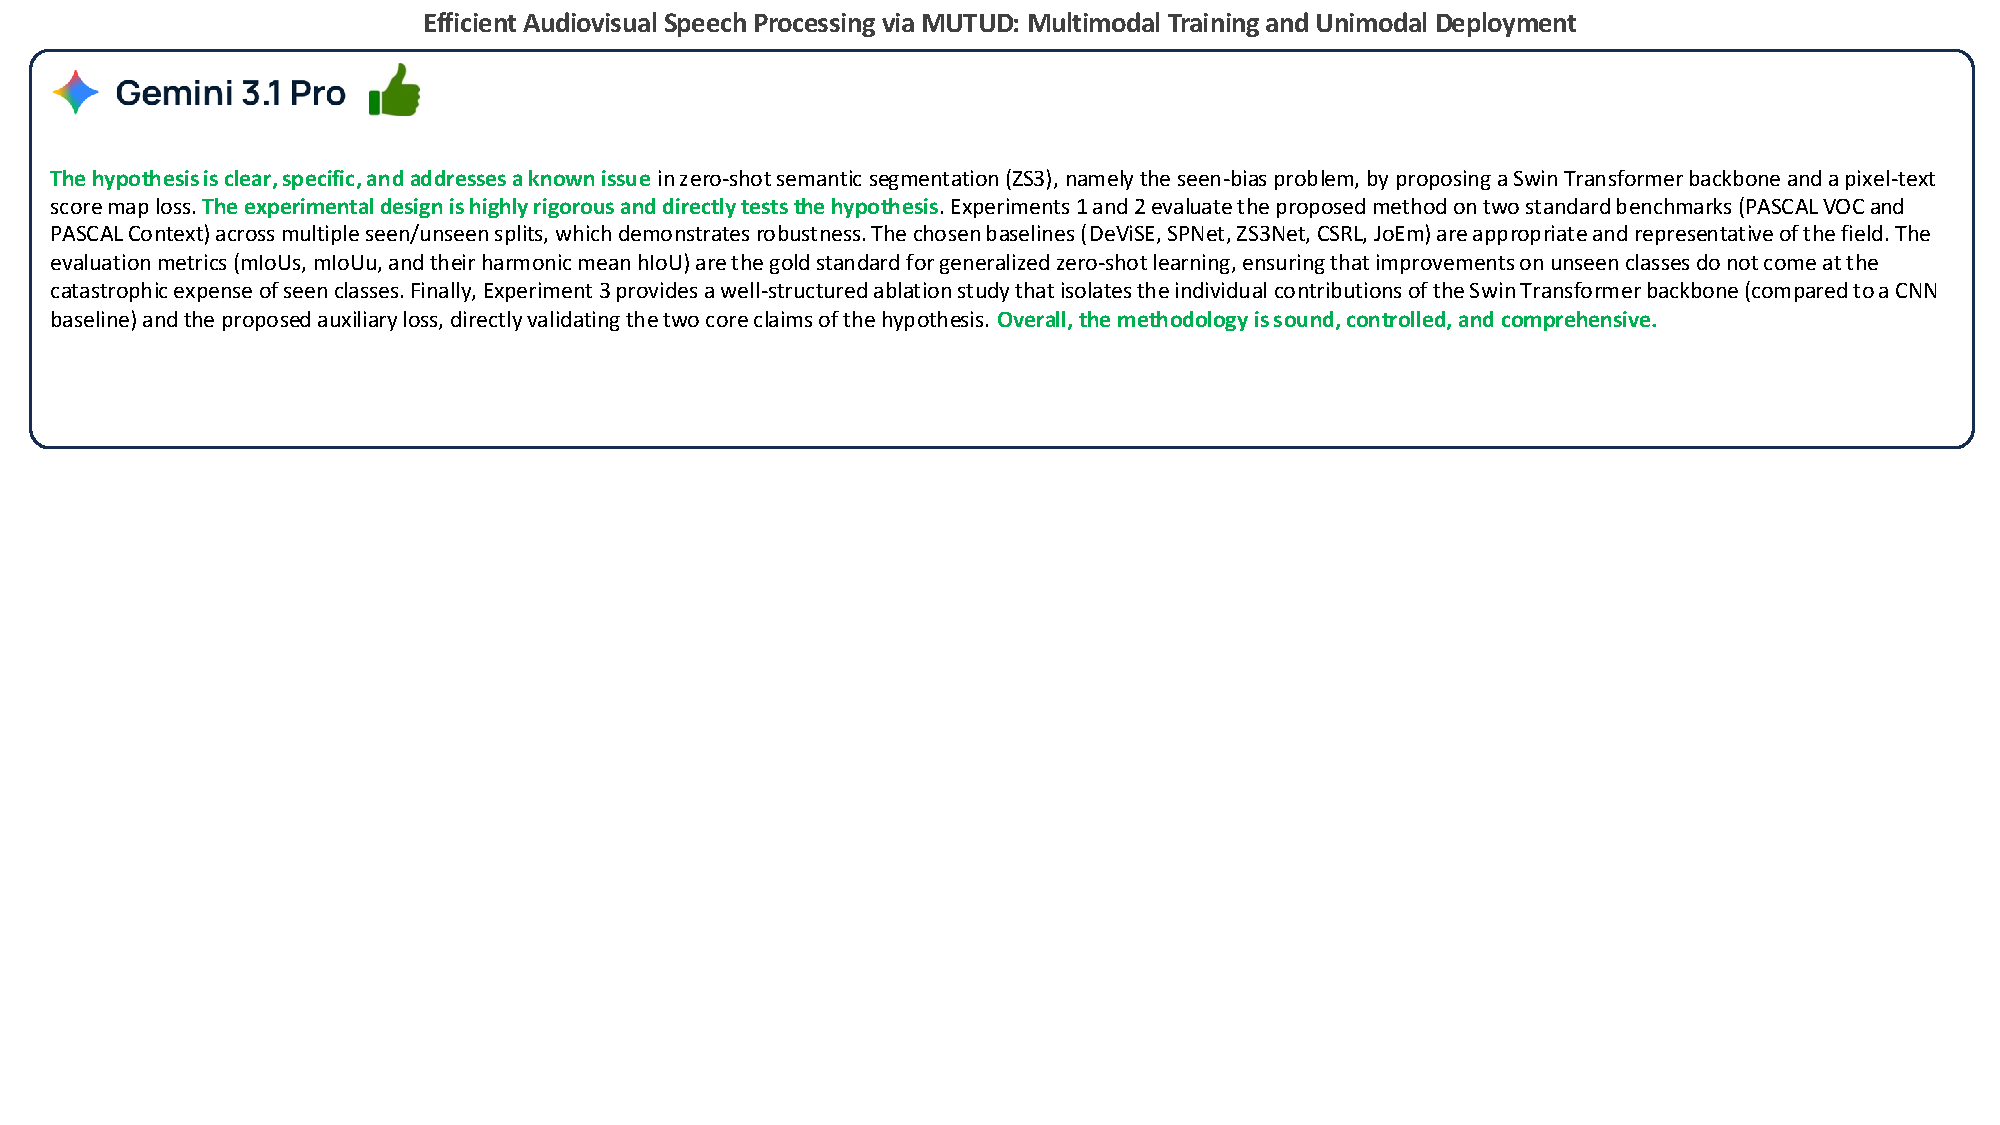
\includegraphics[width=\linewidth,height=0.82\textheight,keepaspectratio]{figures/gemini31-fp.pdf}
    \caption{\textbf{Gemini 3.1 Pro response for the false-positive example in Fig.~\ref{fig:example-fp}.} The model assigns a high-soundness judgment to the low-soundness proposal.}
    \label{fig:example-fp-gemini31-response}
\end{figure}

\begin{figure}[p]
    \centering
    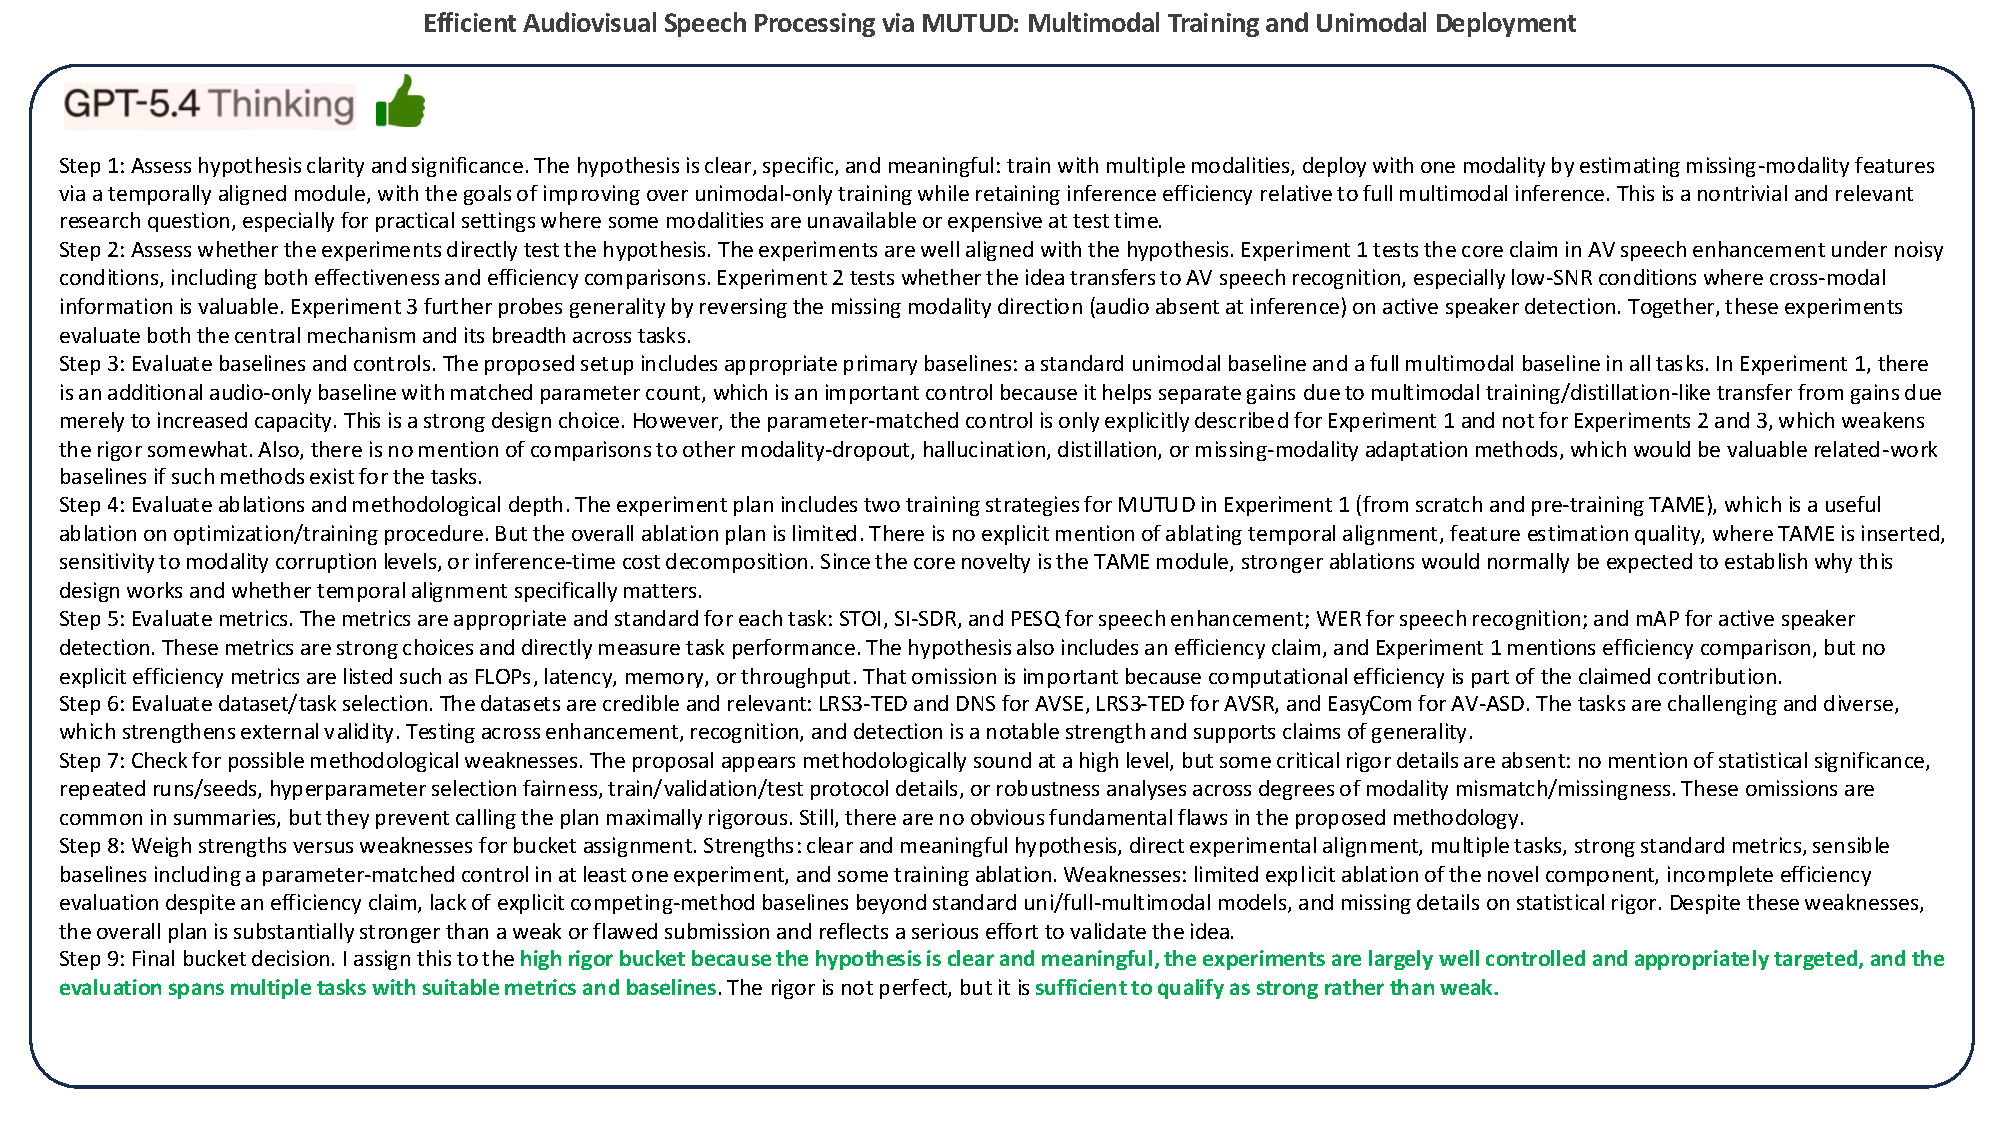
\includegraphics[width=\linewidth,height=0.82\textheight,keepaspectratio]{figures/gpt54-fp.pdf}
    \caption{\textbf{GPT-5.4 Thinking response for the false-positive example in Fig.~\ref{fig:example-fp}.} The model assigns a high-soundness judgment to the low-soundness proposal.}
    \label{fig:example-fp-gpt54-response}
\end{figure}

\begin{figure}[p]
    \centering
    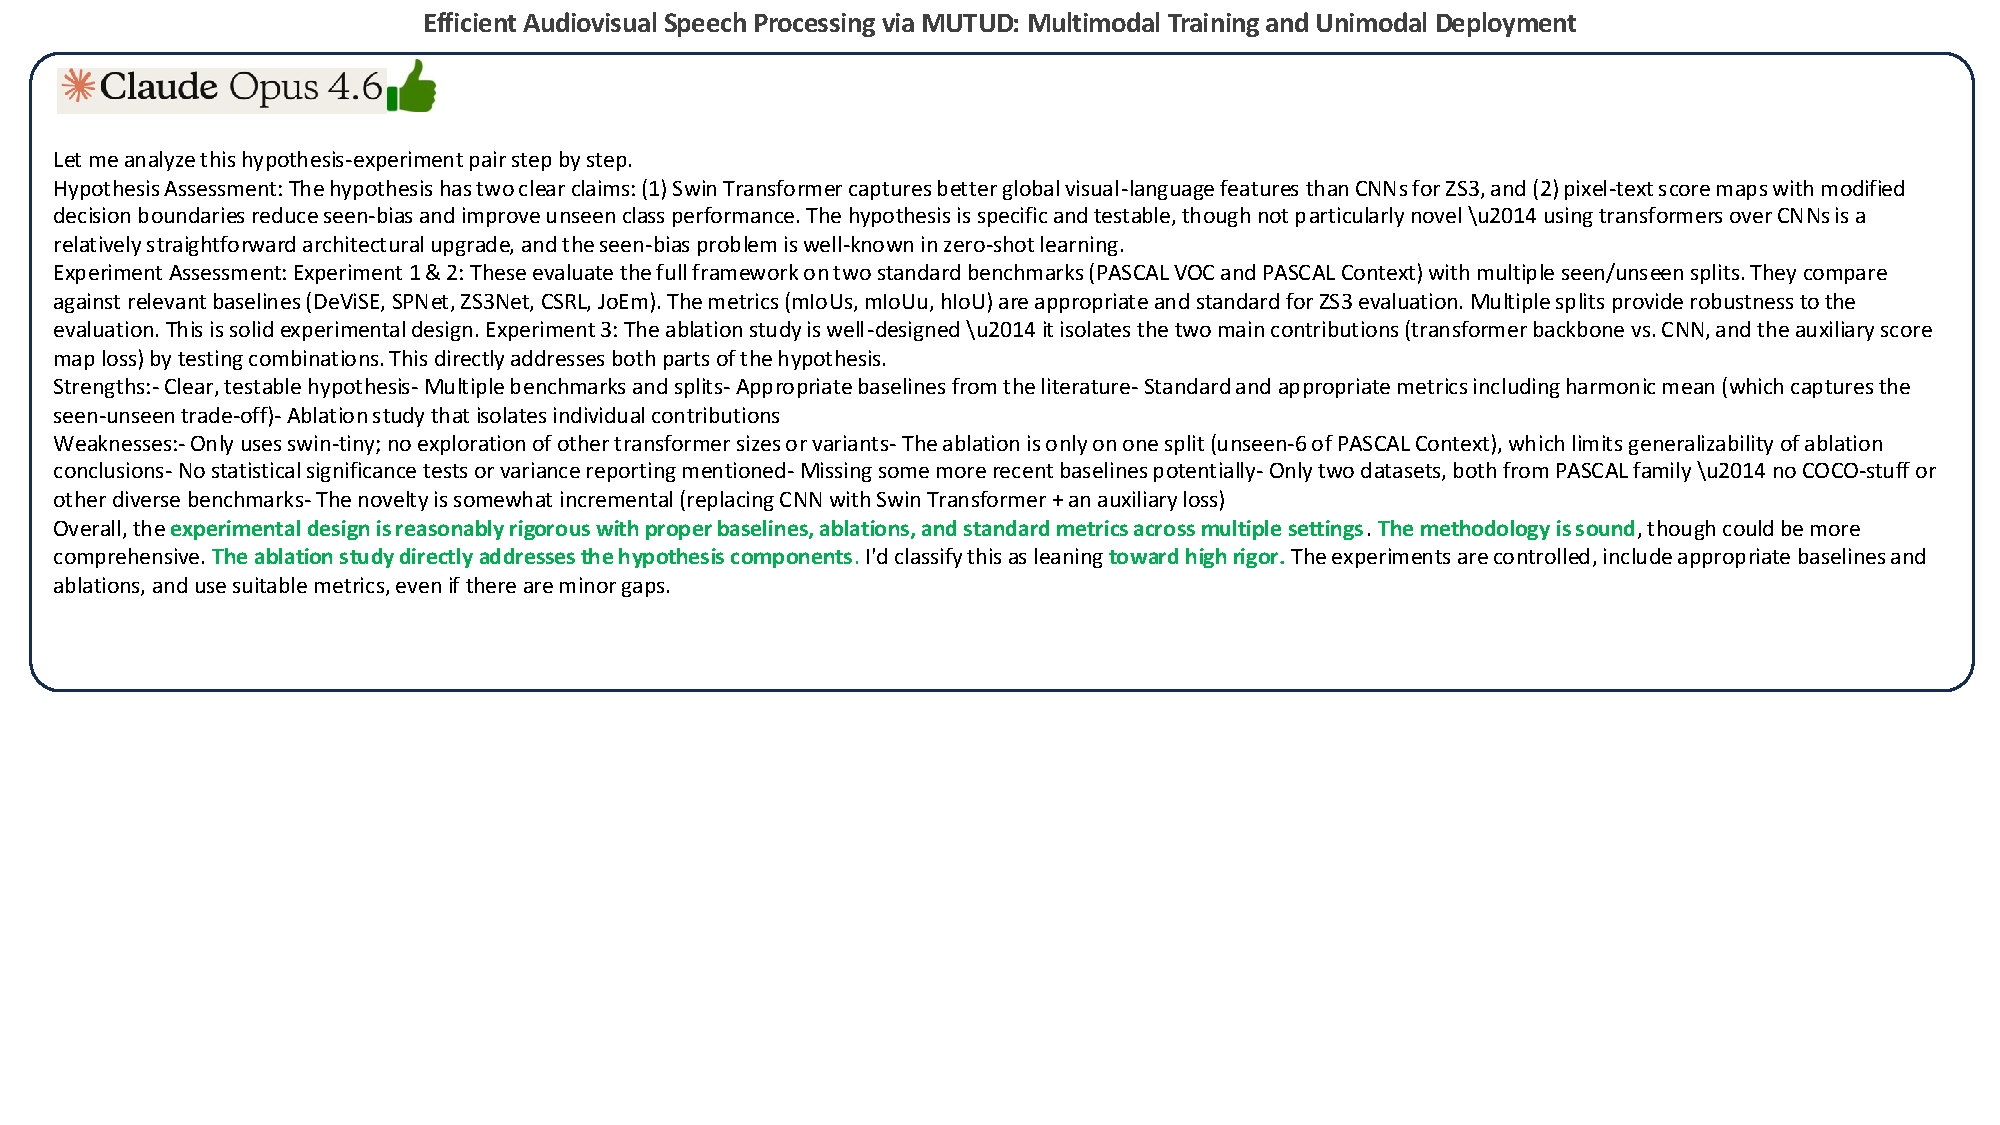
\includegraphics[width=\linewidth,height=0.82\textheight,keepaspectratio]{figures/opus46-fp.pdf}
    \caption{\textbf{Claude Opus 4.6 response for the false-positive example in Fig.~\ref{fig:example-fp}.} The model assigns a high-soundness judgment to the low-soundness proposal.}
    \label{fig:example-fp-opus46-response}
\end{figure}

\begin{figure}[p]
    \centering
    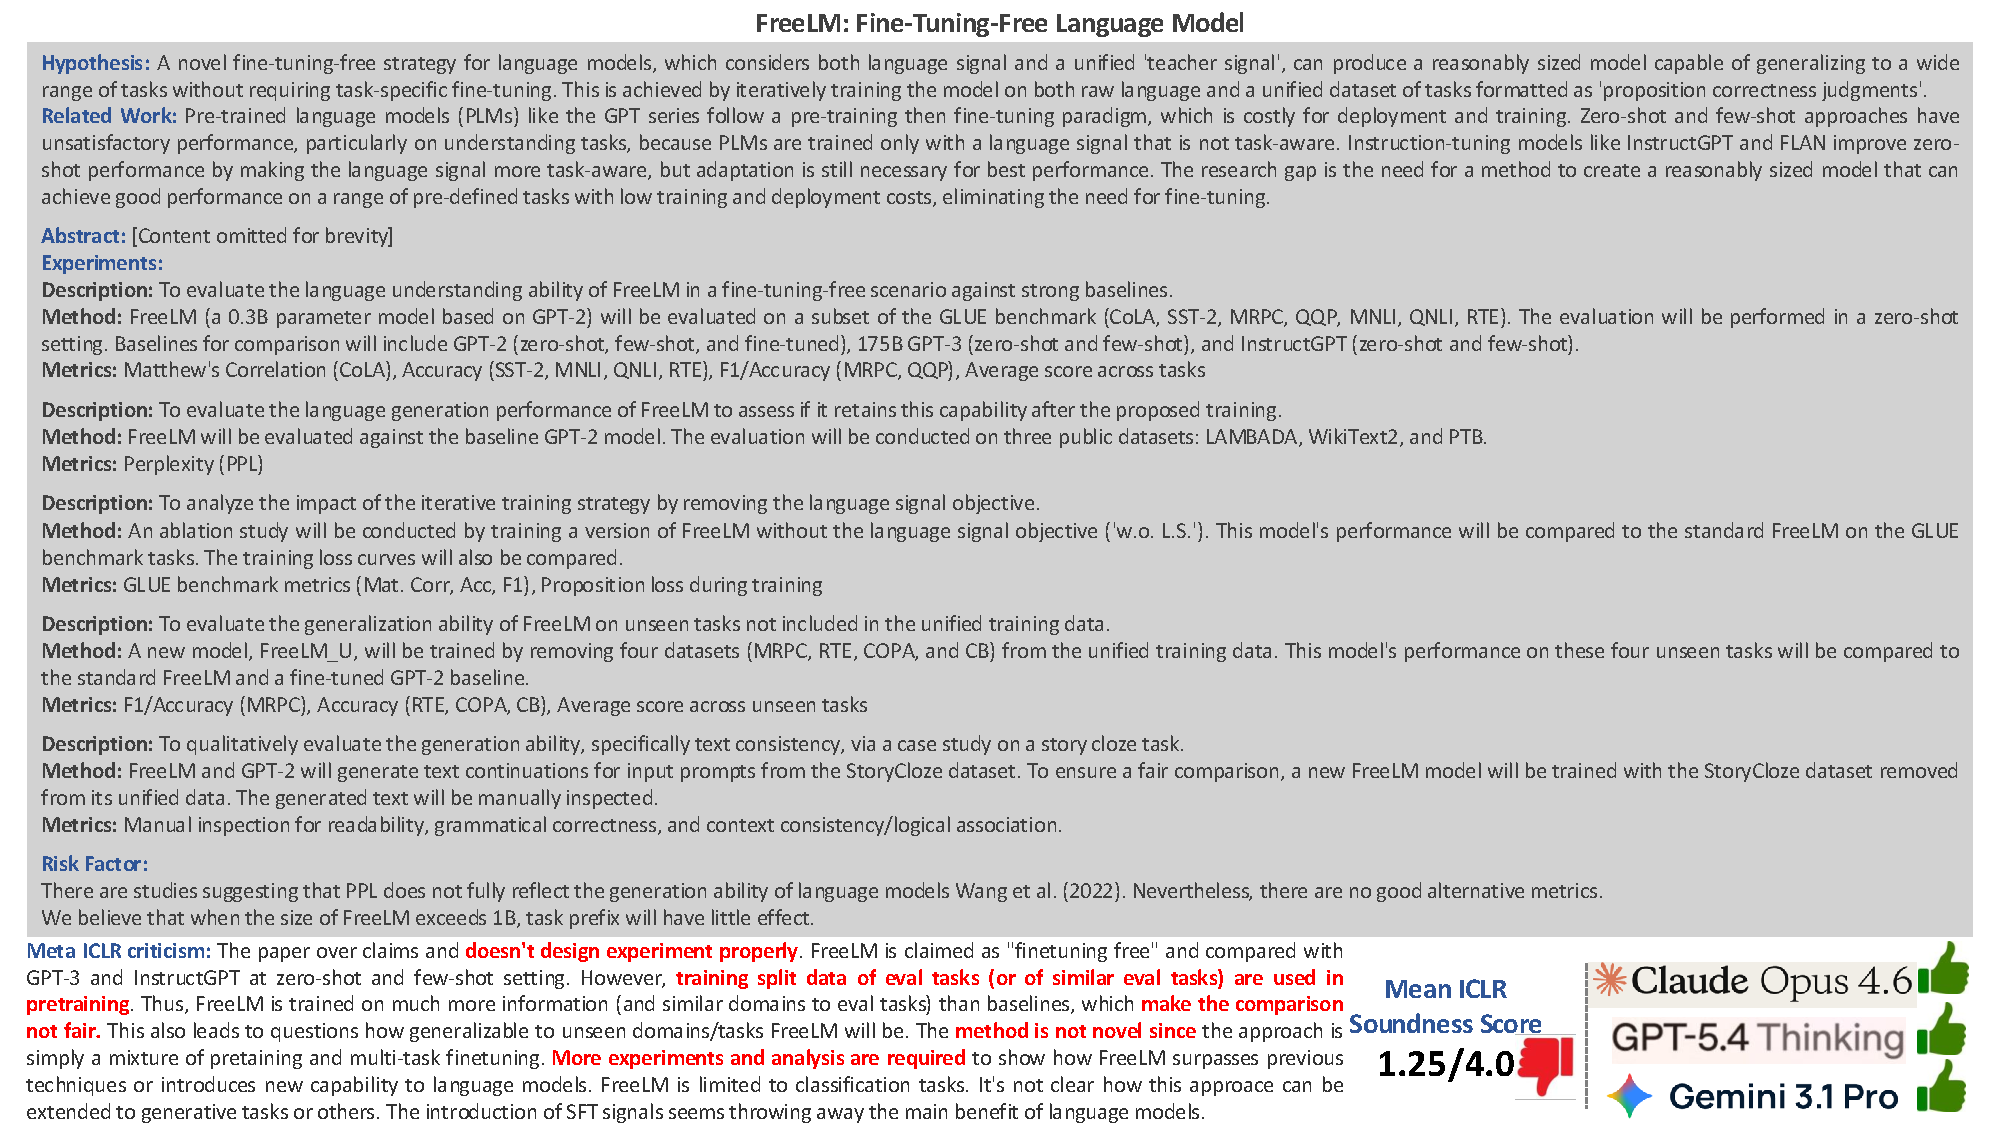
\includegraphics[width=\linewidth]{figures/example-fp-2.pdf}
    \caption{\textbf{Second false-positive example.} A low-soundness proposal is predicted as high soundness by Claude Opus 4.6, GPT-5.4 Thinking, and Gemini 3.1 Pro despite reviewer concerns that the paper overclaims, lacks experimental support, and uses evaluation-task pretraining data that weakens the comparison.}
    \label{fig:example-fp-2}
\end{figure}

\begin{figure}[p]
    \centering
    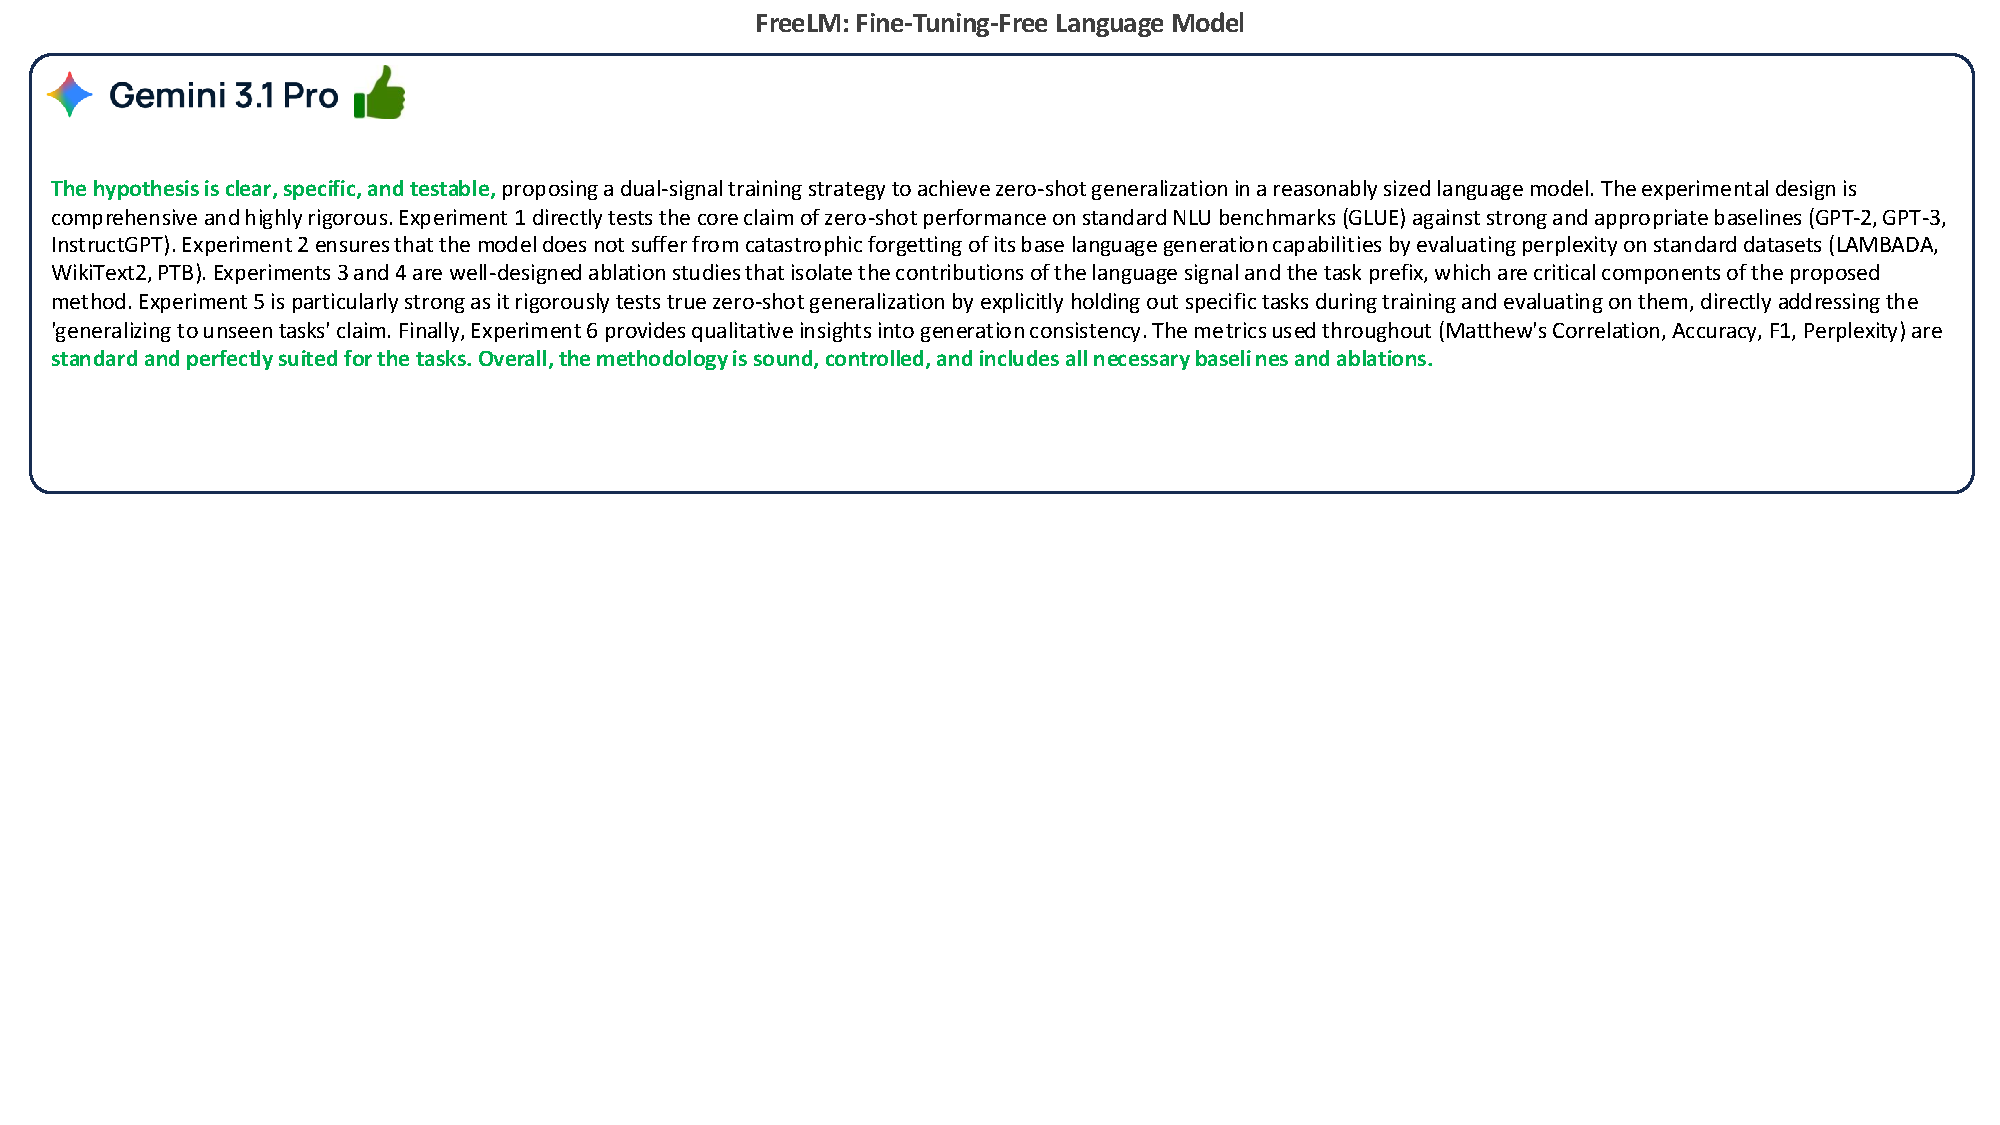
\includegraphics[width=\linewidth,height=0.82\textheight,keepaspectratio]{figures/gemini31-fp-2.pdf}
    \caption{\textbf{Gemini 3.1 Pro response for the second false-positive example in Fig.~\ref{fig:example-fp-2}.} The model assigns a high-soundness judgment to the low-soundness proposal.}
    \label{fig:example-fp-2-gemini31-response}
\end{figure}

\begin{figure}[p]
    \centering
    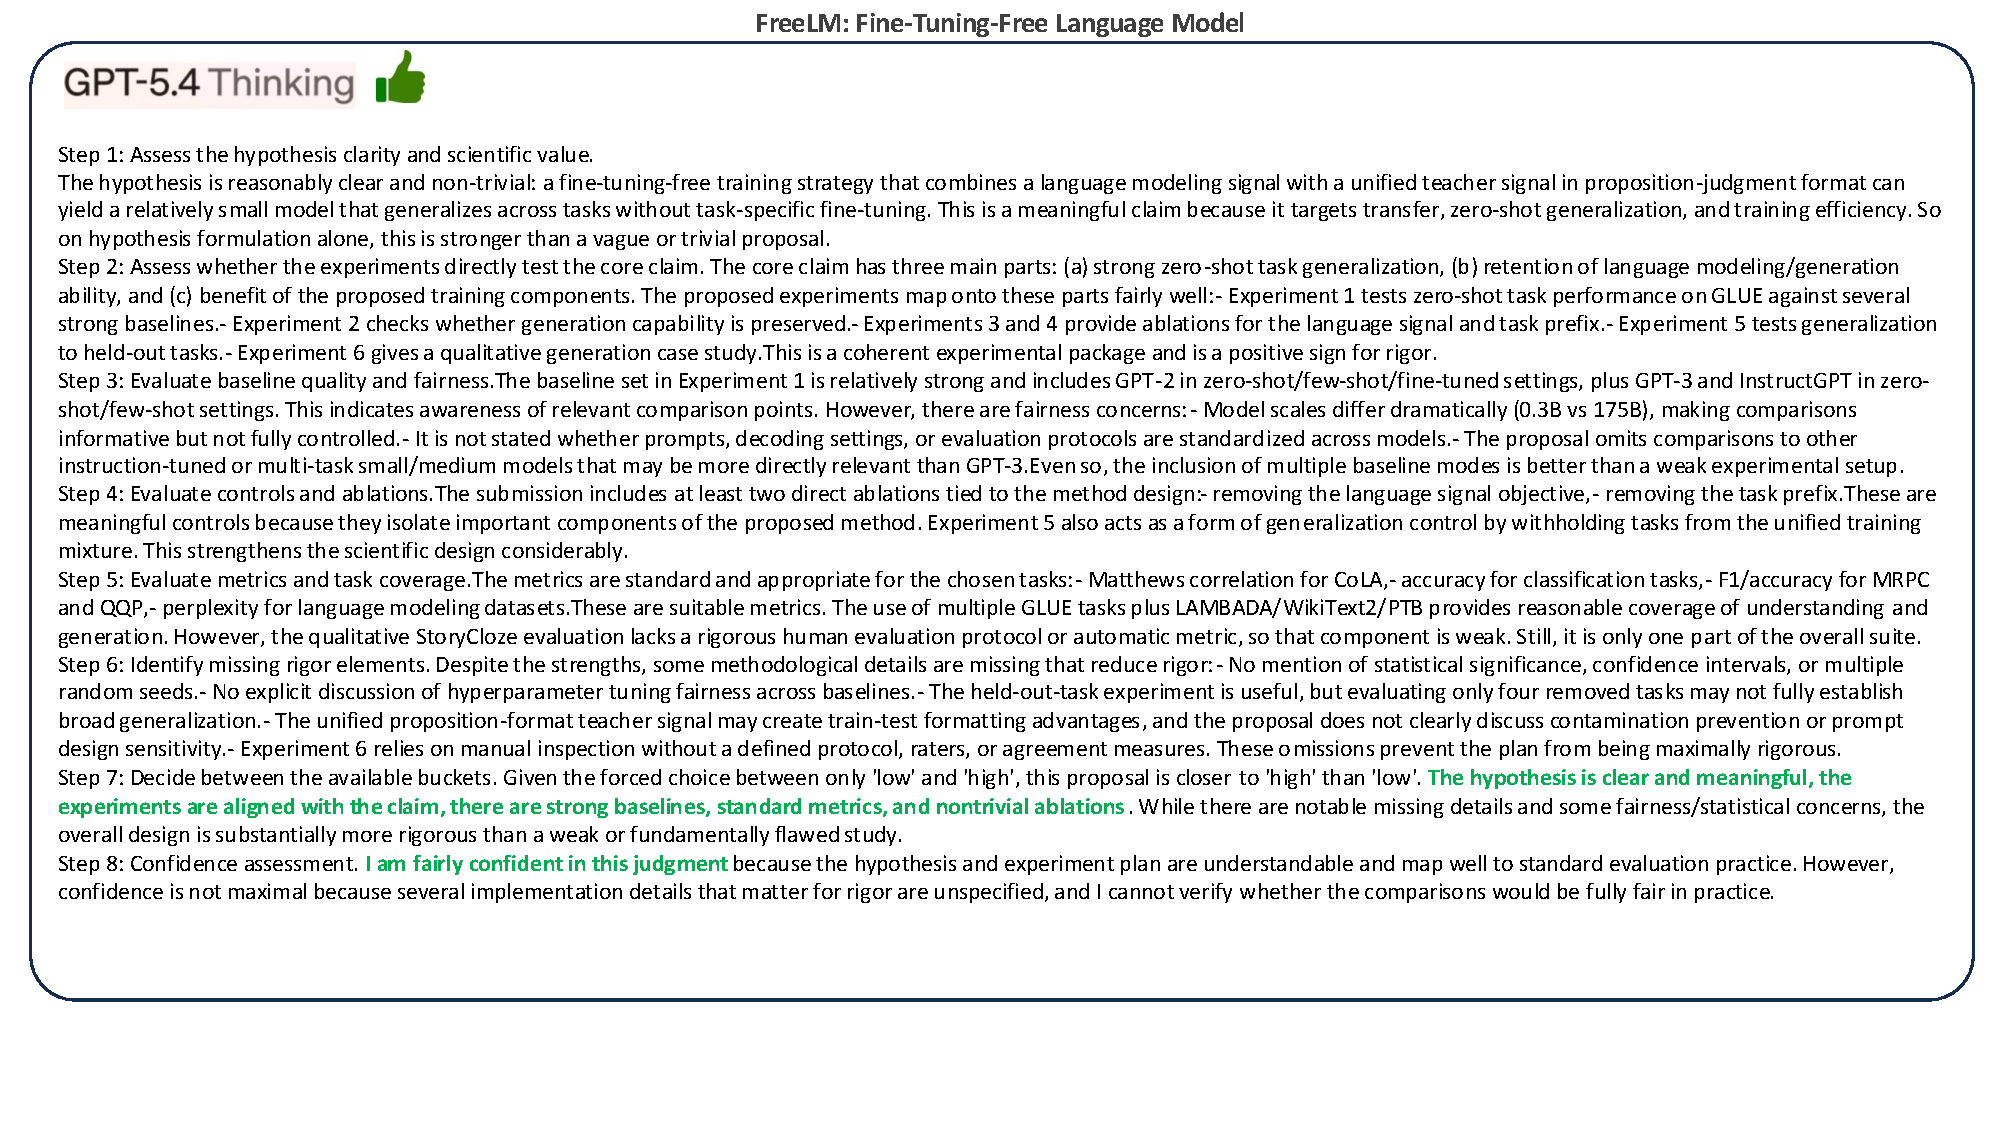
\includegraphics[width=\linewidth,height=0.82\textheight,keepaspectratio]{figures/gpt54-fp-2.pdf}
    \caption{\textbf{GPT-5.4 Thinking response for the second false-positive example in Fig.~\ref{fig:example-fp-2}.} The model assigns a high-soundness judgment to the low-soundness proposal.}
    \label{fig:example-fp-2-gpt54-response}
\end{figure}

\begin{figure}[p]
    \centering
    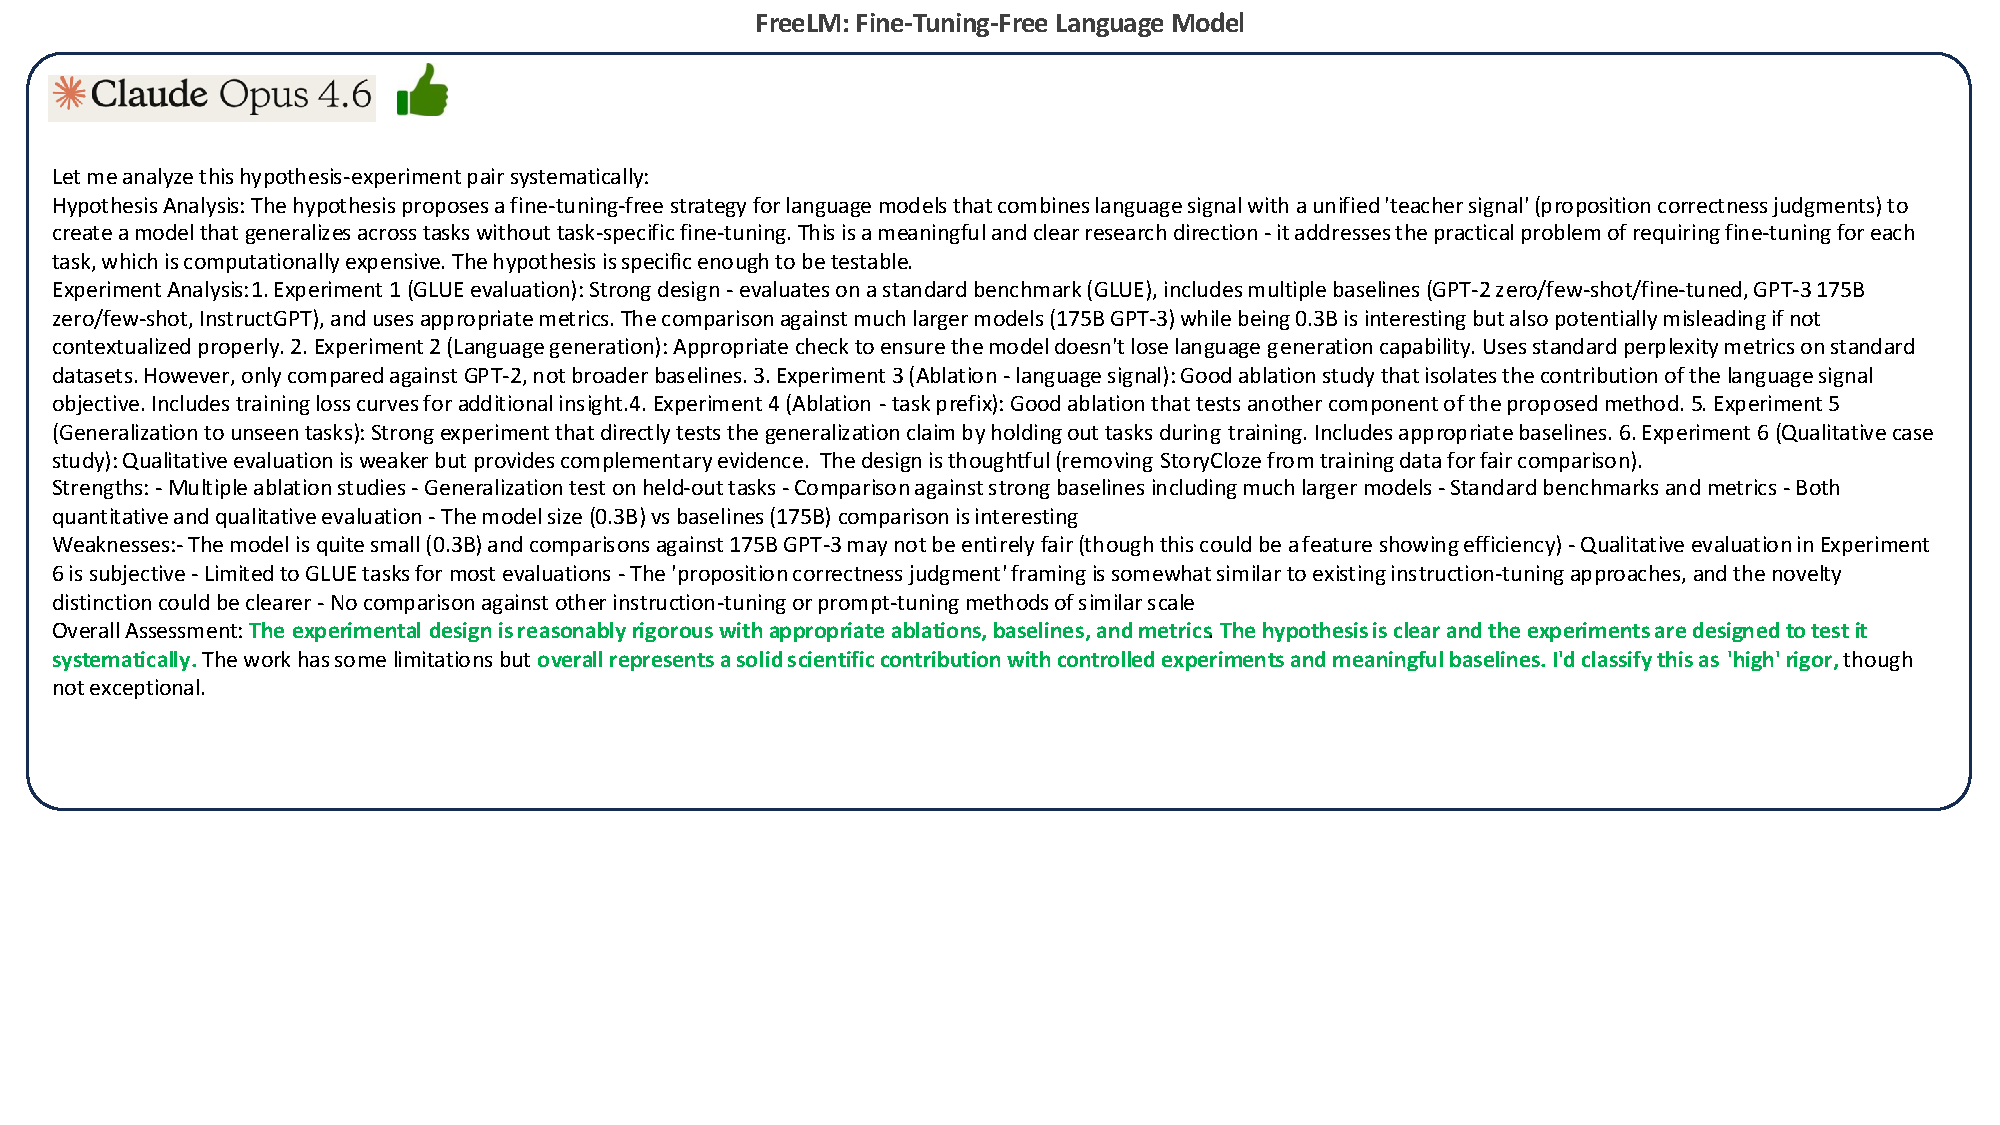
\includegraphics[width=\linewidth,height=0.82\textheight,keepaspectratio]{figures/opus46-fp-2.pdf}
    \caption{\textbf{Claude Opus 4.6 response for the second false-positive example in Fig.~\ref{fig:example-fp-2}.} The model assigns a high-soundness judgment to the low-soundness proposal.}
    \label{fig:example-fp-2-opus46-response}
\end{figure}

\begin{figure}[p]
    \centering
    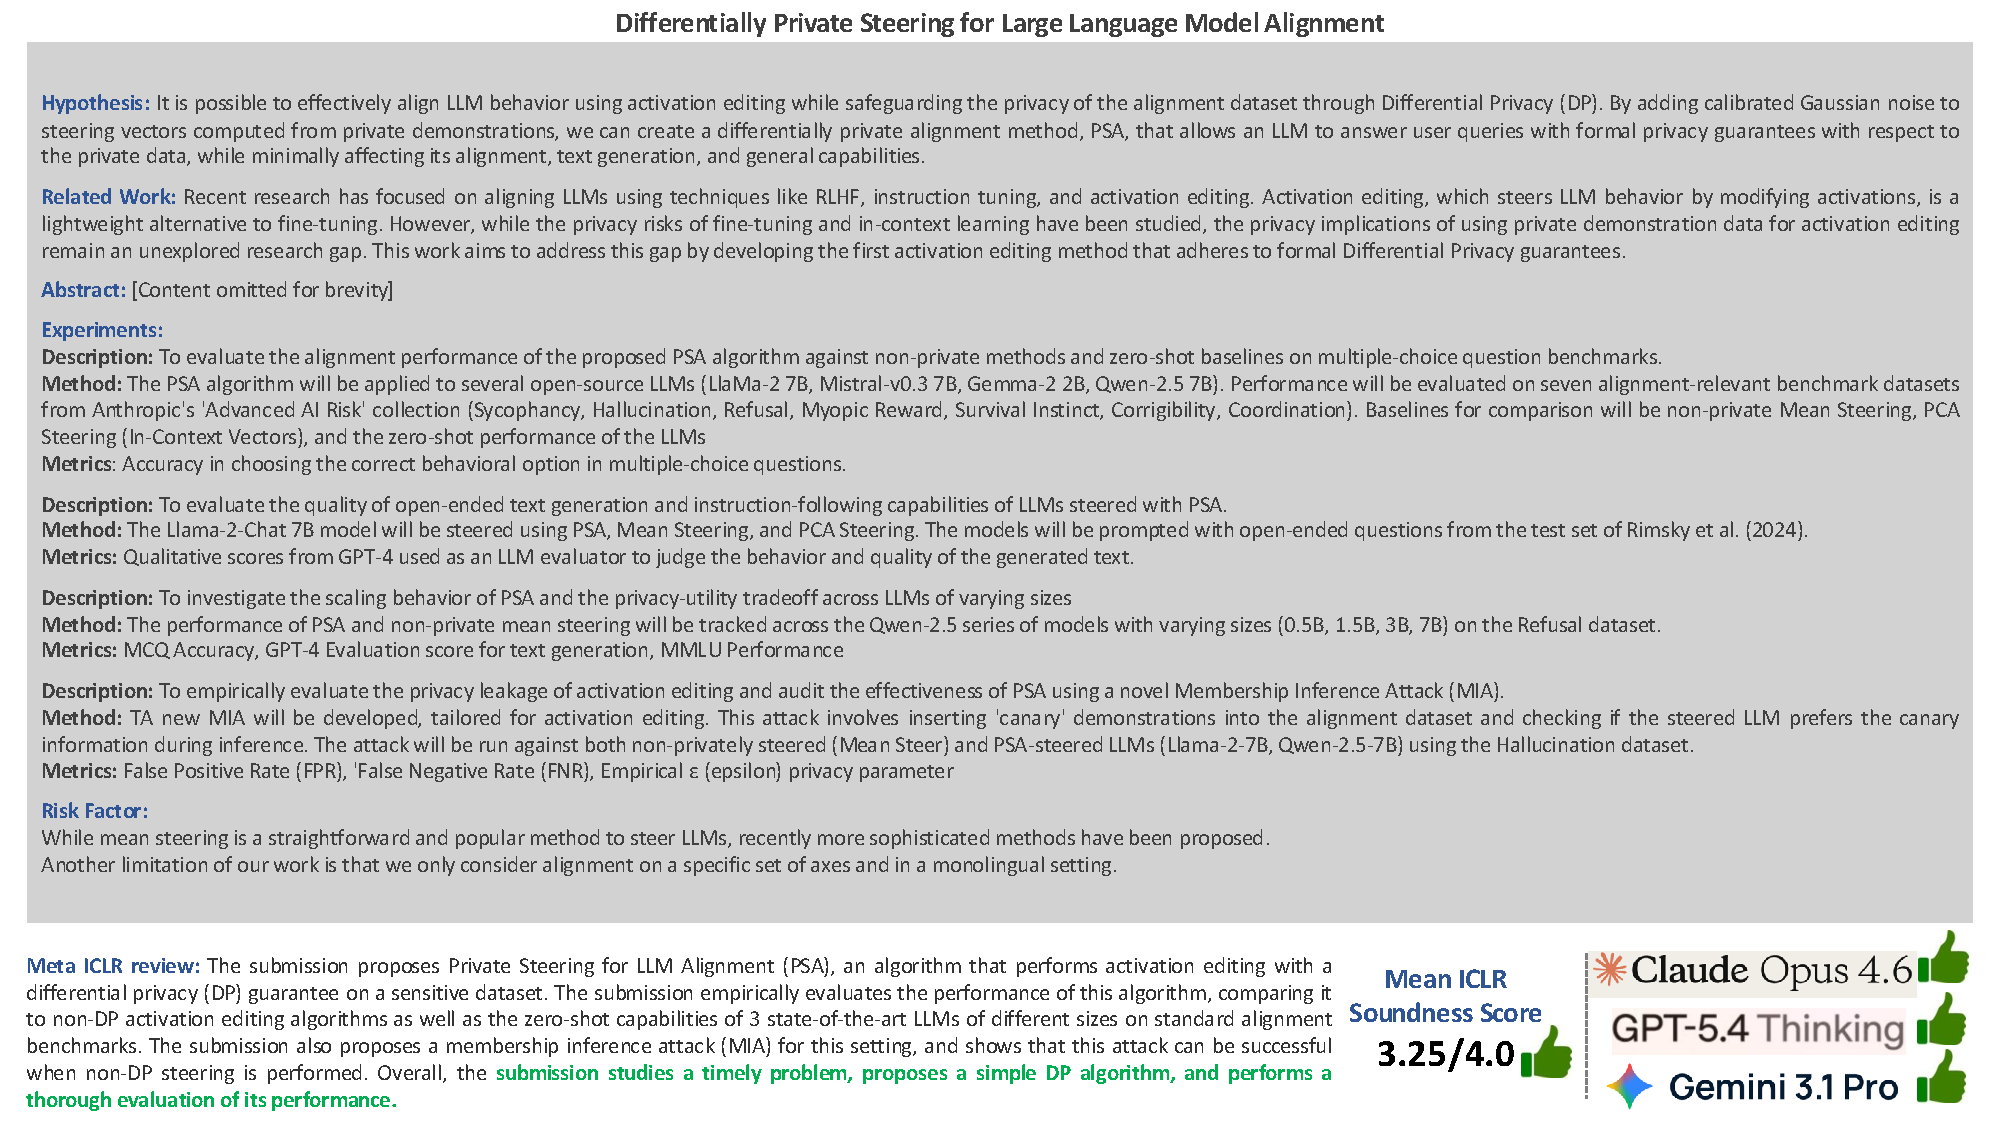
\includegraphics[width=\linewidth]{figures/example-tp.pdf}
    \caption{\textbf{True-positive example.} A high-soundness proposal is correctly predicted as high soundness by Claude Opus 4.6, GPT-5.4 Thinking, and Gemini 3.1 Pro, matching the favorable reviewer assessment of the proposed method and evaluation plan.}
    \label{fig:example-tp}
\end{figure}

\begin{figure}[p]
    \centering
    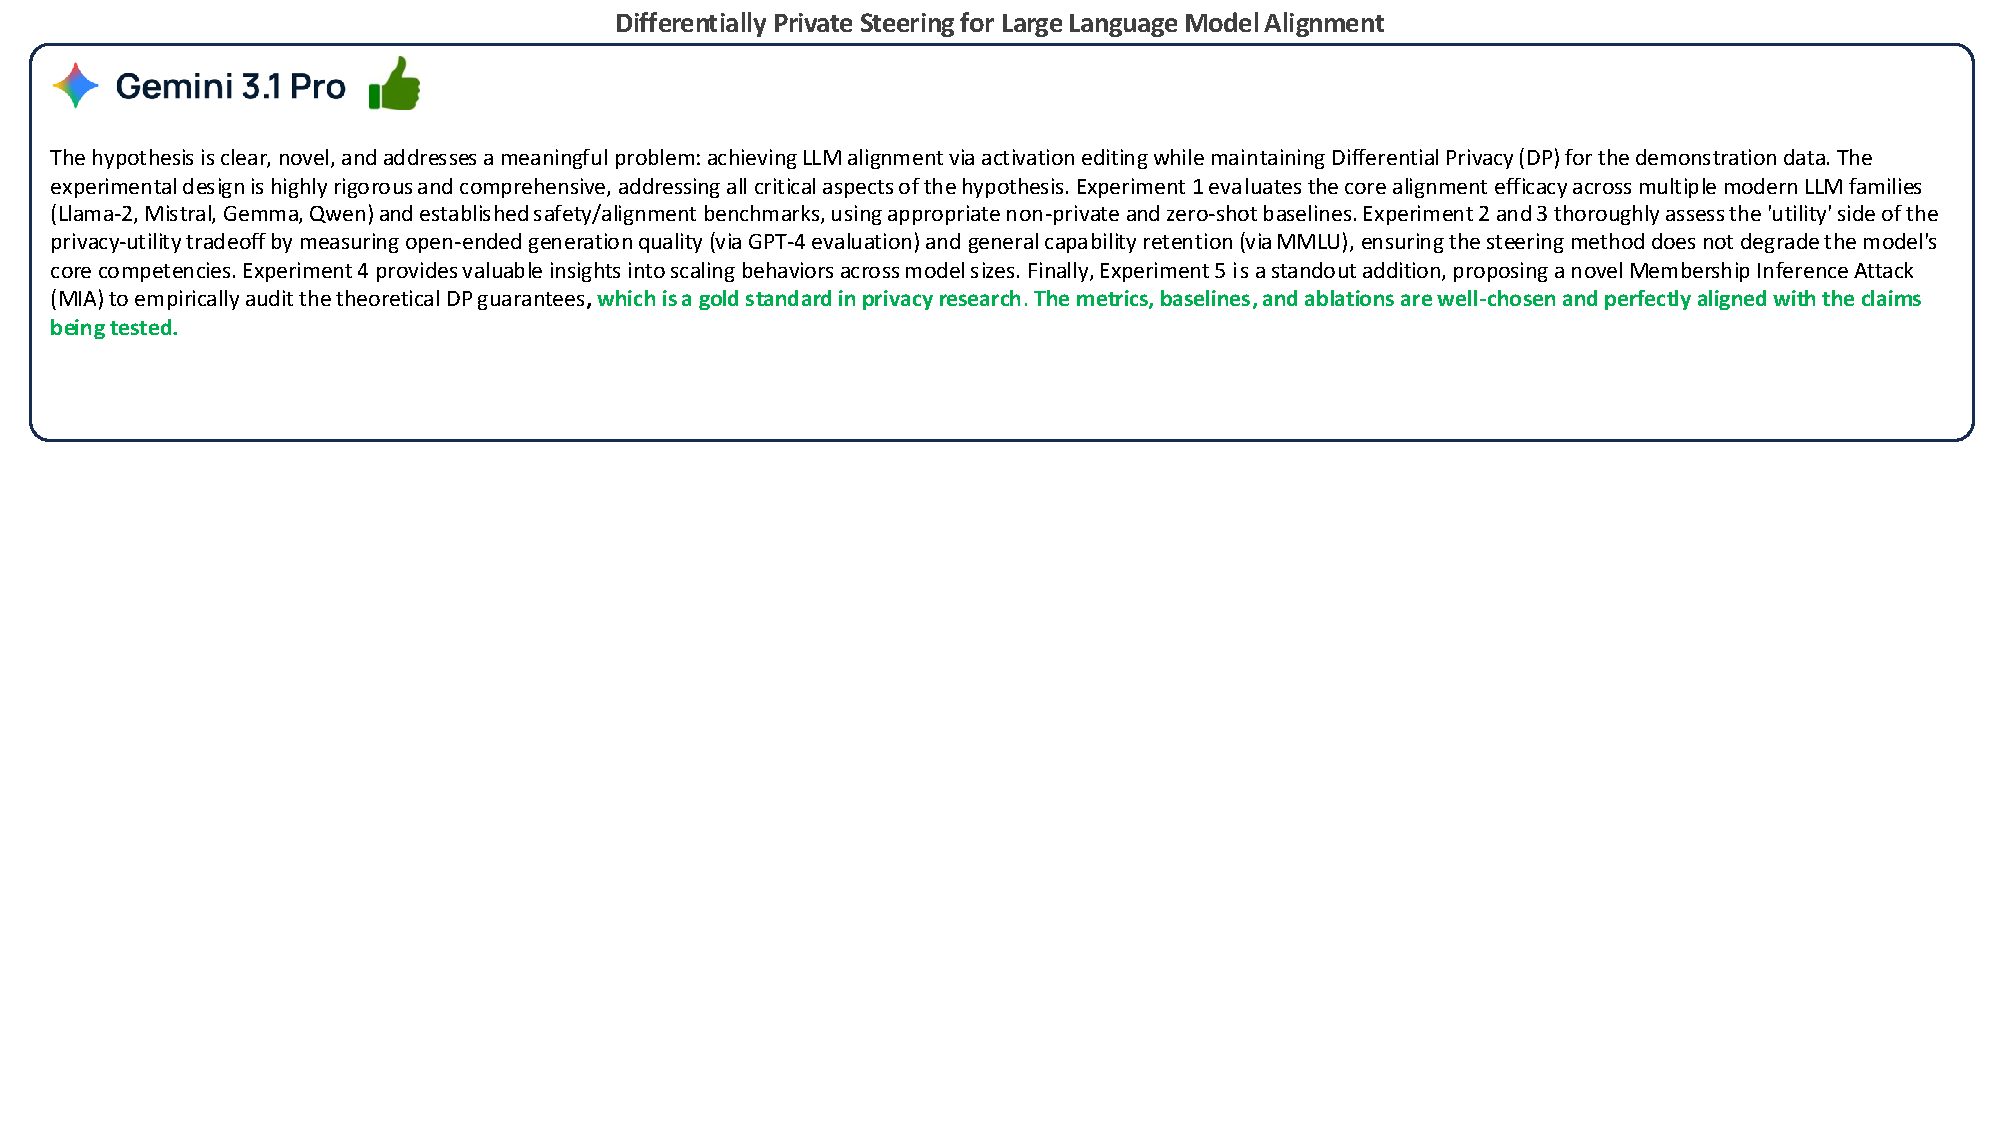
\includegraphics[width=\linewidth,height=0.82\textheight,keepaspectratio]{figures/gemini31-tp.pdf}
    \caption{\textbf{Gemini 3.1 Pro response for the true-positive example in Fig.~\ref{fig:example-tp}.} The model assigns a high-soundness judgment to the high-soundness proposal.}
    \label{fig:example-tp-gemini31-response}
\end{figure}

\begin{figure}[p]
    \centering
    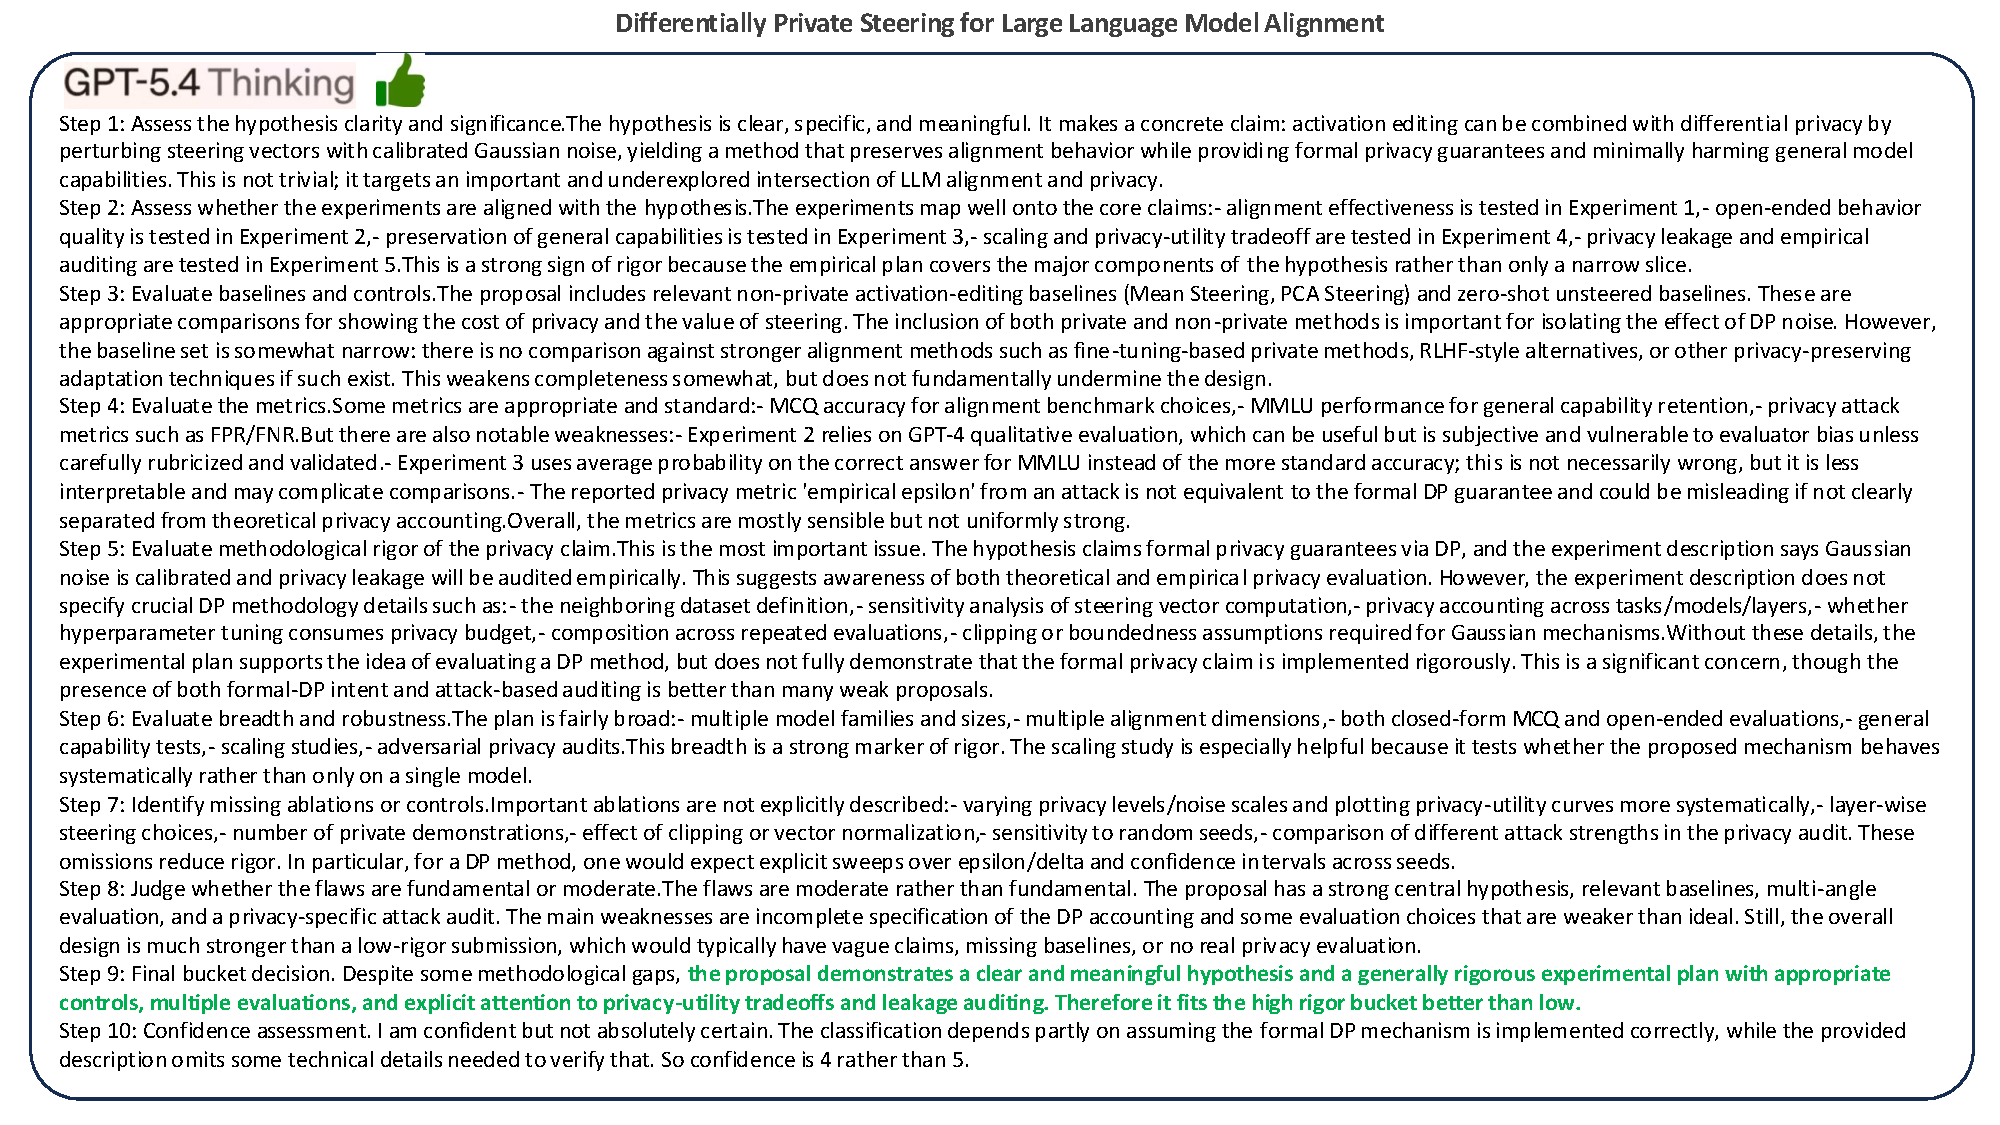
\includegraphics[width=\linewidth,height=0.82\textheight,keepaspectratio]{figures/gpt54-tp.pdf}
    \caption{\textbf{GPT-5.4 Thinking response for the true-positive example in Fig.~\ref{fig:example-tp}.} The model assigns a high-soundness judgment to the high-soundness proposal.}
    \label{fig:example-tp-gpt54-response}
\end{figure}

\begin{figure}[p]
    \centering
    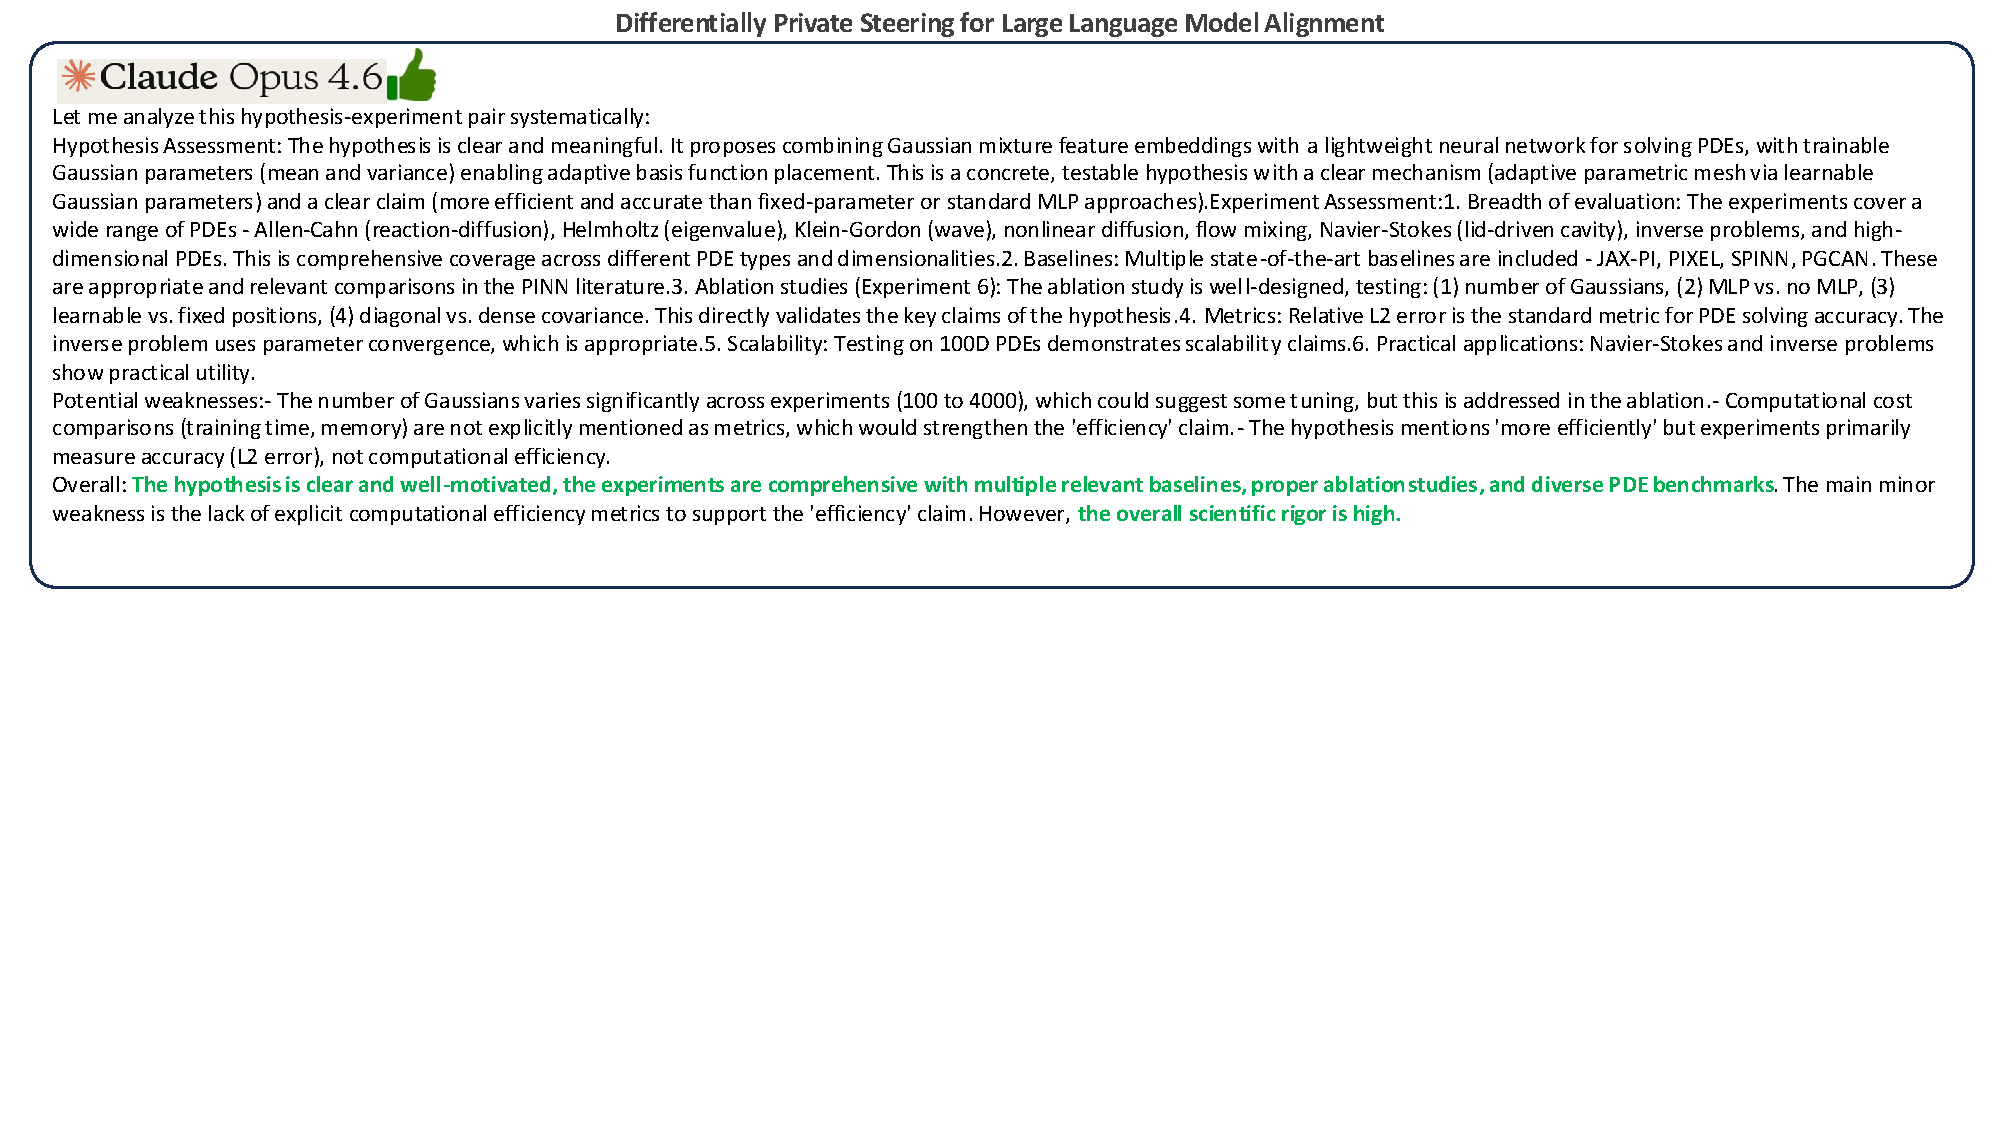
\includegraphics[width=\linewidth,height=0.82\textheight,keepaspectratio]{figures/opus46-tp.pdf}
    \caption{\textbf{Claude Opus 4.6 response for the true-positive example in Fig.~\ref{fig:example-tp}.} The model assigns a high-soundness judgment to the high-soundness proposal.}
    \label{fig:example-tp-opus46-response}
\end{figure}
